\section*{Analysis}
%% Our basic analysis is based on the following three measures:
%% \begin{itemize}[]
%% \item \textbf{Trajectory graph.} This plots the change of the article
%%   over time. By measuring a levenshtein distance between each revision
%%   text against the final version (see algorithm~\ref{traj-calc}), we
%%   see the article in terms of its growth from an empty article, and
%%   the approach to its final version. We also plot the size of the
%%   article at each point of this graph for greater context.
%% \item \textbf{User by share.} We sum up each user's 'share' of the
%%   article using the calculations made during analysis, and order them
%%   here by user.
%% \item \textbf{User by edit count.} Our understanding of the previous
%%   graph can be made greater if we understand how many edits each user
%%   has made.
%% \end{itemize}
\subsection*{Share and edit count plots}
We find two typical, unweighted edit graphs in
figure~\ref{fig:average-share}.

\begin{figure}
  \centering
  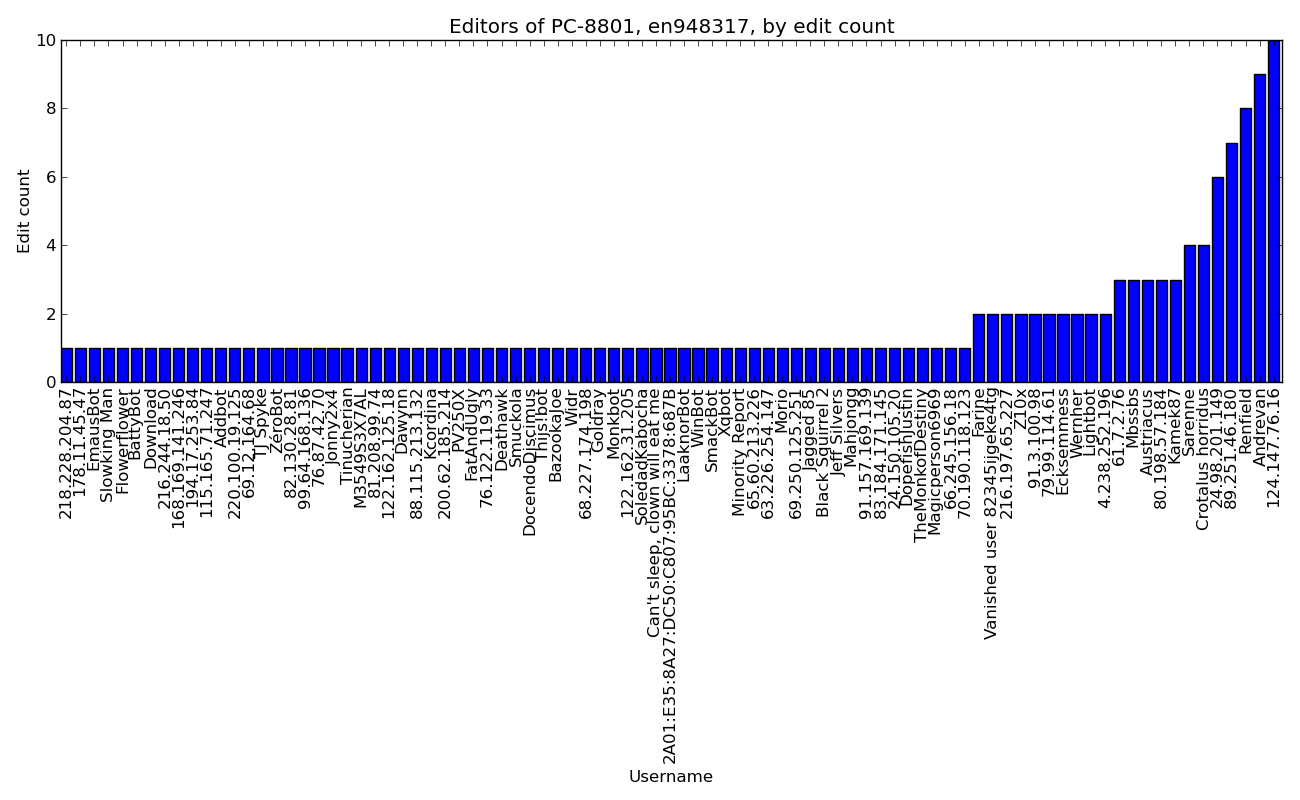
\includegraphics[width=1\linewidth]{img/editshare/pc8801count.png}
  \newline
  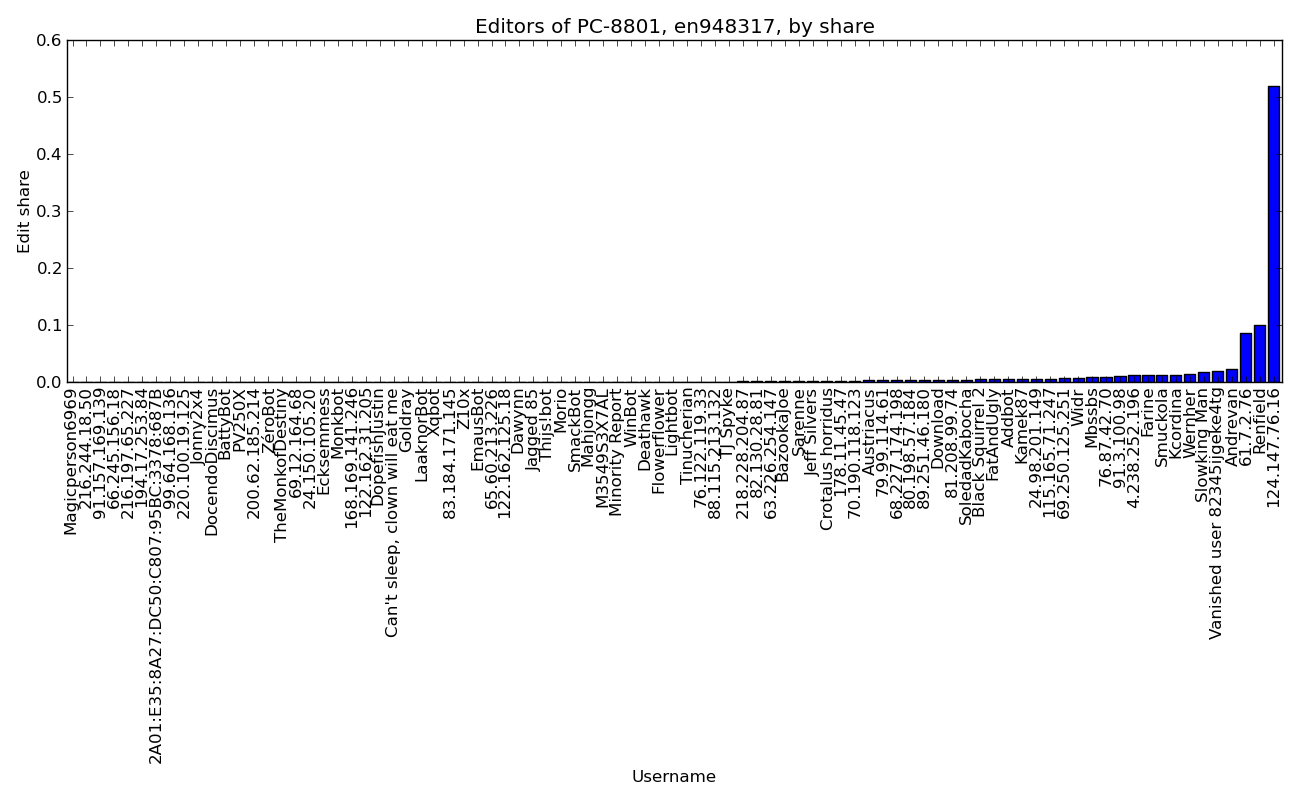
\includegraphics[width=1\linewidth]{img/editshare/pc8801share.png}
  \caption{English Wikipedia, Page ID 948317 (PC-8801), user graphs}
  \label{fig:average-share}
\end{figure}

These two graphs are typical of the data set on the whole, showing
many one-time editors, with a small amount of repeat editors. More
similar graphs are found in appendix~\ref{sec:edit-share}.

We can note here that a lot of the single-time entries are anonymous,
showing an IP address rather than a user-name. Since IP addresses are
likely to change (it is standard practice for a ISP to provide a new
IP address for their customers on each new connection), we cannot know
how many separate agents these IP addresses represent. We can't
necessarily be sure that the 10-edit user is one person either, but
for the purposes of this study this isn't an issue.

We can also find our first bots on these graphs, with many making
small numbers of edits. EmausBot towards the left of the edit count
graph, BattyBot next -- it is common practice to name the bot account
with an obvious bot-name. Emausbot comes up a lot in our analyses, in
fact. It maintains inter-wiki links.

From our first graphs we found that many articles, particularly in
smaller Wikipedias have little-to-no edits, and would result in graphs
like the one in figure~\ref{fig:useless-share}. For this reason, when
fetching random articles, we automatically discard a revision if it
falls below a certain threshold revision-count.

\begin{wrapfigure}{i}{0.4\linewidth}
  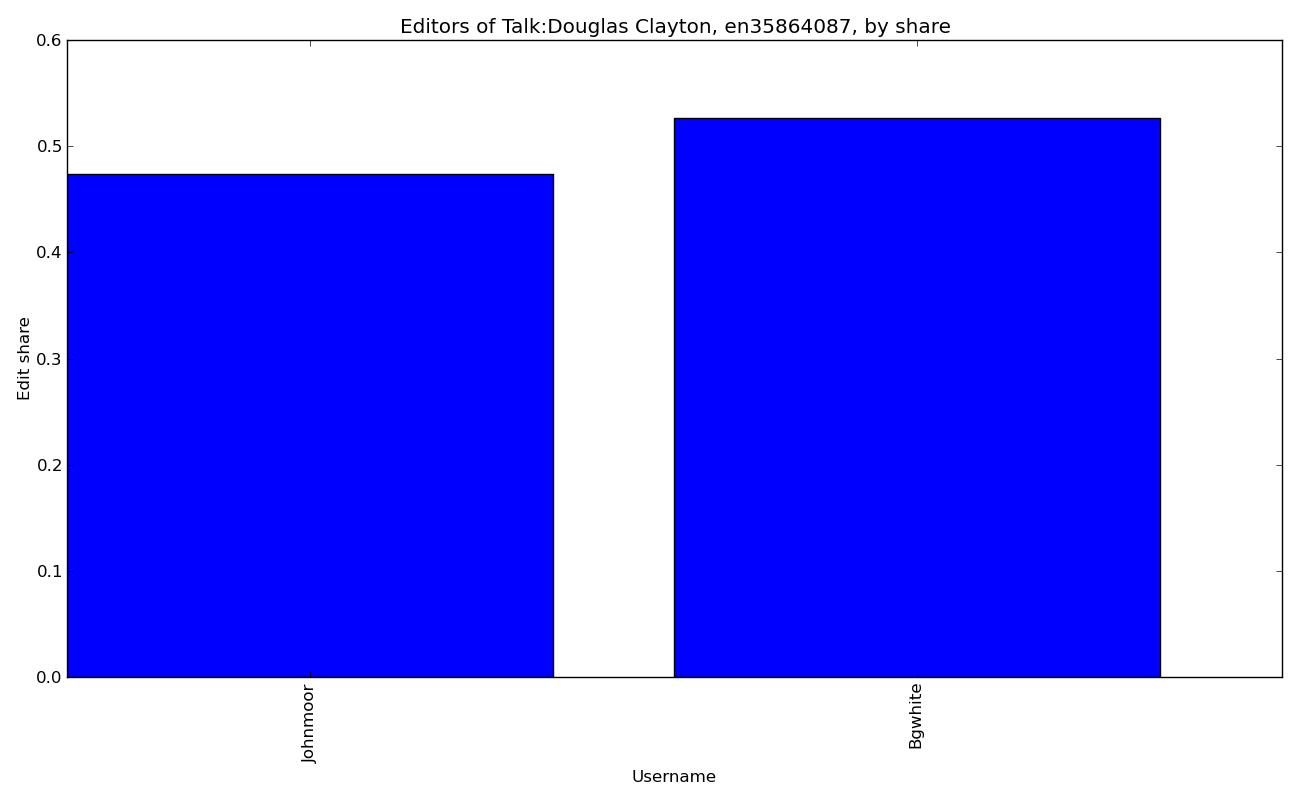
\includegraphics[width=1\linewidth]{img/useless/Talk:DouglasClayton.png}
  \caption{English Wikipedia, Page ID 35864087 (Talk:Douglas
    Clayton), share}
  \label{fig:useless-share}
\end{wrapfigure}

We also experimented with automatic, arbitrary weight setting to see
how the graph would be effected. We see one such example in
figure~\ref{fig:one-weight}, where we contrast an unweighted data set,
with one where we double the weight of the `links' weight.

In this case, in fact, it was doubling the links value that created
the most dramatic change. Changing maths, files/images, structure and
normal text weights created the least change -- all the graphs can be
found in appendix~\ref{sec:LudvigFadeev} for comparison.

\begin{figure}
  \makebox[\linewidth][c]{
    \begin{subfigure}[b!]{0.6\linewidth}
      \centering
      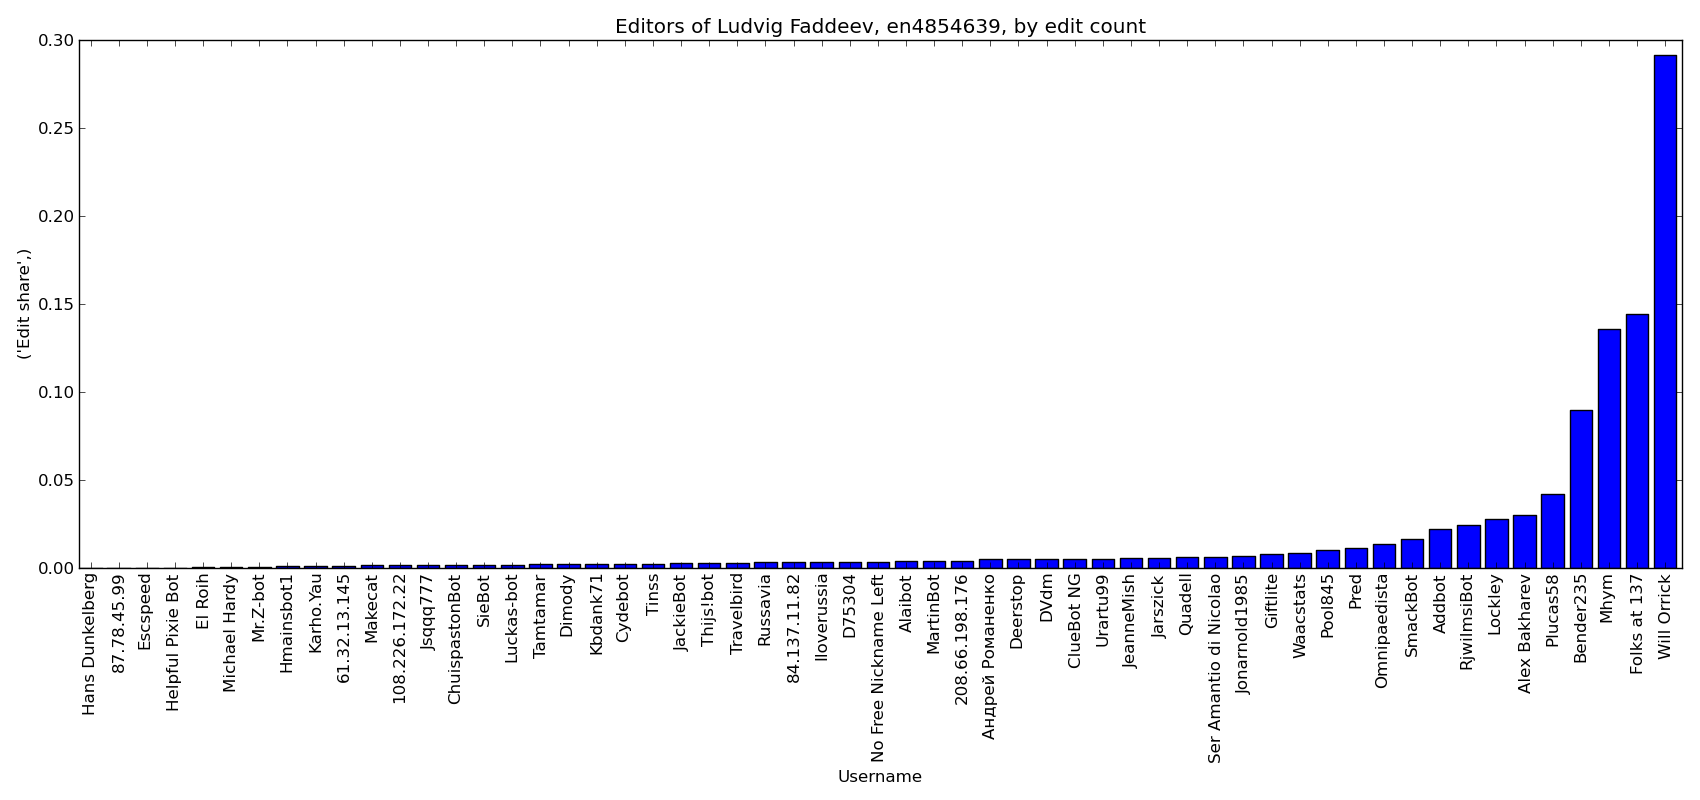
\includegraphics[width=\linewidth]{img/weightings/LudvigFaddeevUnweighted.png}
      \caption{Unweighted share}
    \end{subfigure}
    \begin{subfigure}[b!]{0.6\linewidth}
      \centering
      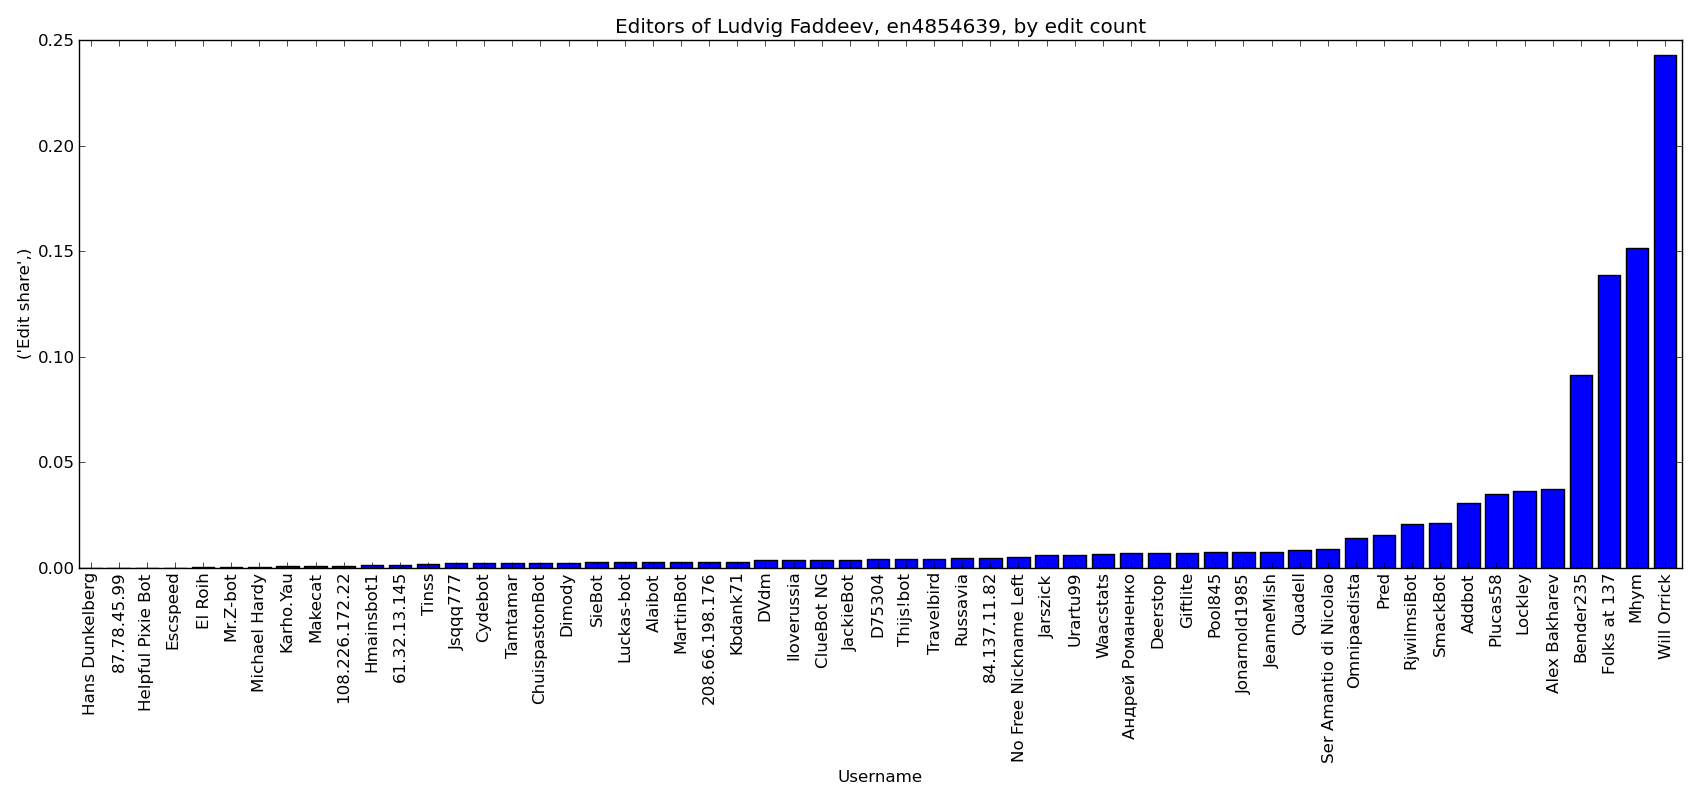
\includegraphics[width=\linewidth]{img/weightings/LudvigFaddeevLinks.png}
      \caption{Share with doubly-weight links}
    \end{subfigure}
  }
  \caption{English Wikipedia, Page ID 4854639 (Ludvig Faddeev)}
  \label{fig:one-weight}
\end{figure}

All the graphs we have looked at so far do not take our gradient
factor into account. The effect is interesting when we activate the
gradient factor. Multiplying each summed weights by the gradient
factor as we calculate share, the two graphs in
figure~\ref{fig:one-weight} are transformed into those in
figure~\ref{fig:one-weight-gradient}. The graphs are notably skewed
towards those with the most reward already.

\begin{figure}
  \makebox[\linewidth][c]{
    \begin{subfigure}[b!]{0.6\linewidth}
      \centering
      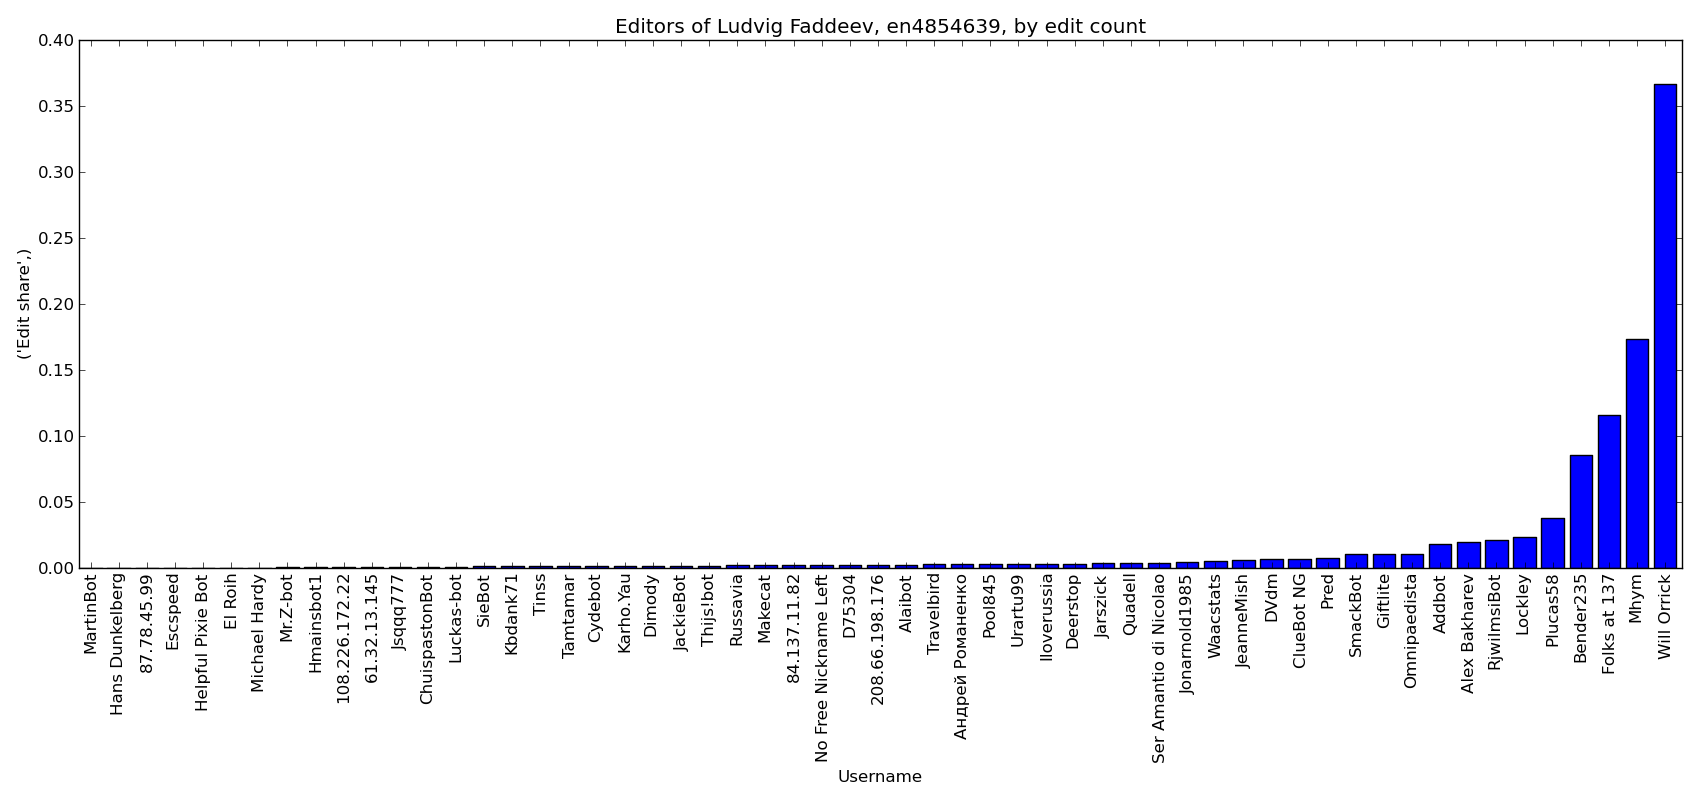
\includegraphics[width=\linewidth]{img/weightings/LudvigFaddeevUnweightedGradient.png}
      \caption{Unweighted share, with gradient factor}
    \end{subfigure}
    \begin{subfigure}[b!]{0.6\linewidth}
      \centering
      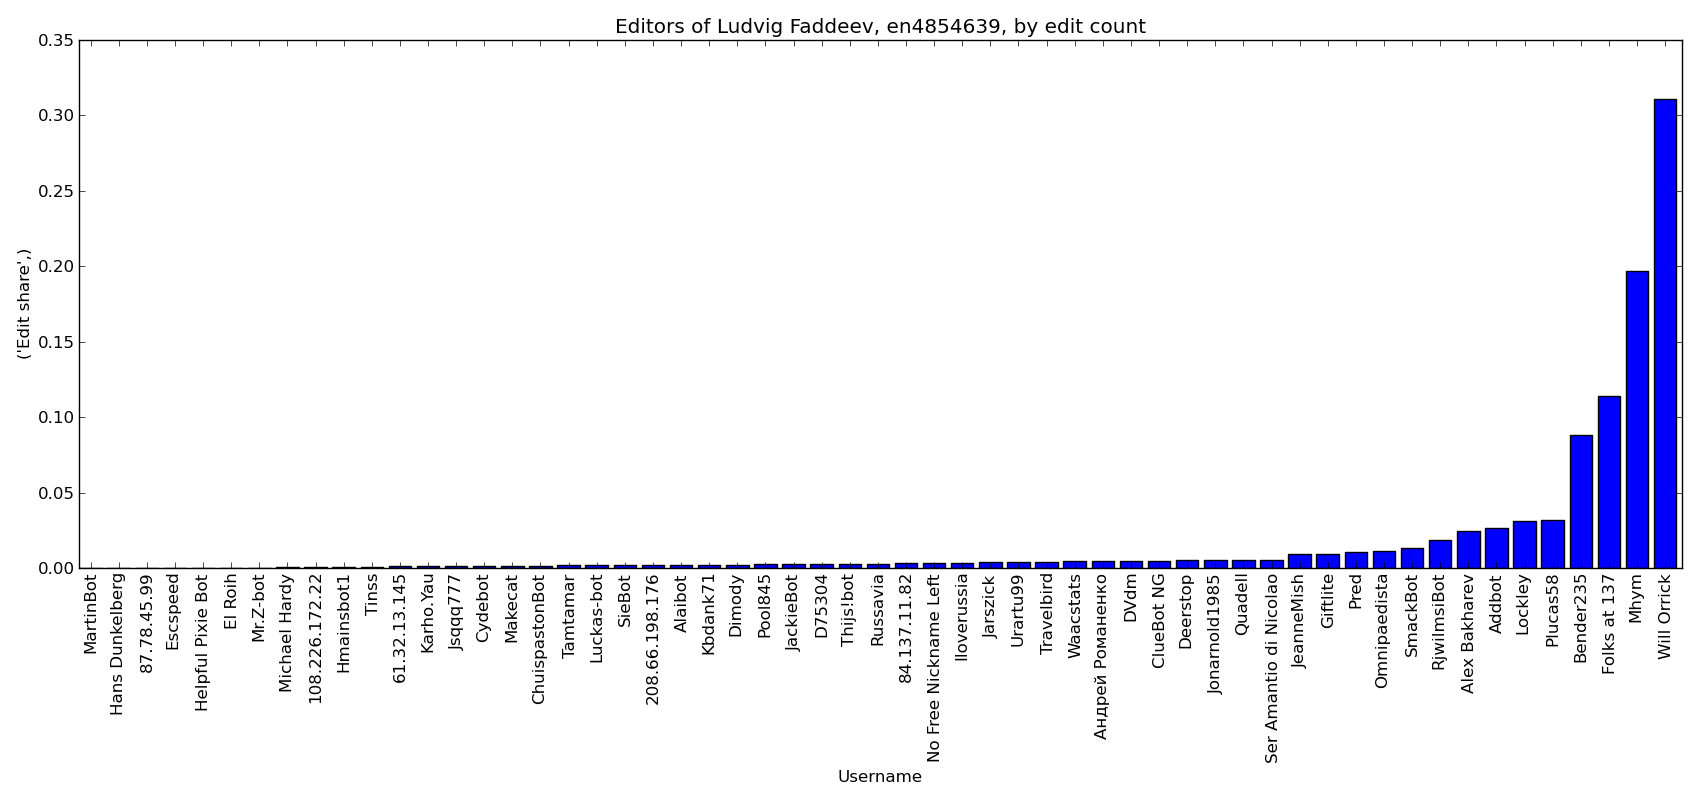
\includegraphics[width=\linewidth]{img/weightings/LudvigFaddeevLinksGradient.png}
      \caption{Share with doubly-weight links and gradient factor}
    \end{subfigure}
  }
  \caption{English Wikipedia, Page ID 4854639 (Ludvig Faddeev)}
  \label{fig:one-weight-gradient}
\end{figure}

\subsection*{Trajectory plots}
On average, these plots follow a similar pattern: the Levenshtein
distance of the article begins at a high value at $x=0$, it's creation
date, and approaches the final article state at $y=0$ and a high value
of $x$. The article begins in a near-empty state, and as it grows,
becomes more and more similar to the final version, before finally
reaching $0$ distance-from-final. 

In the simplest cases, the growth of the article is a rough
mirror-image of the distance-to-final, beginning at the origin and
rising. A few of these `classic' examples can be found in
figure~\ref{fig:traj-classic}. These graphs show a reasonably steady
approach of the final state, increasing in size in a fairly simple
way.

\begin{figure}
  \centering
  \makebox[\linewidth][c]{
    \begin{subfigure}[b!]{0.6\linewidth}
      \centering
      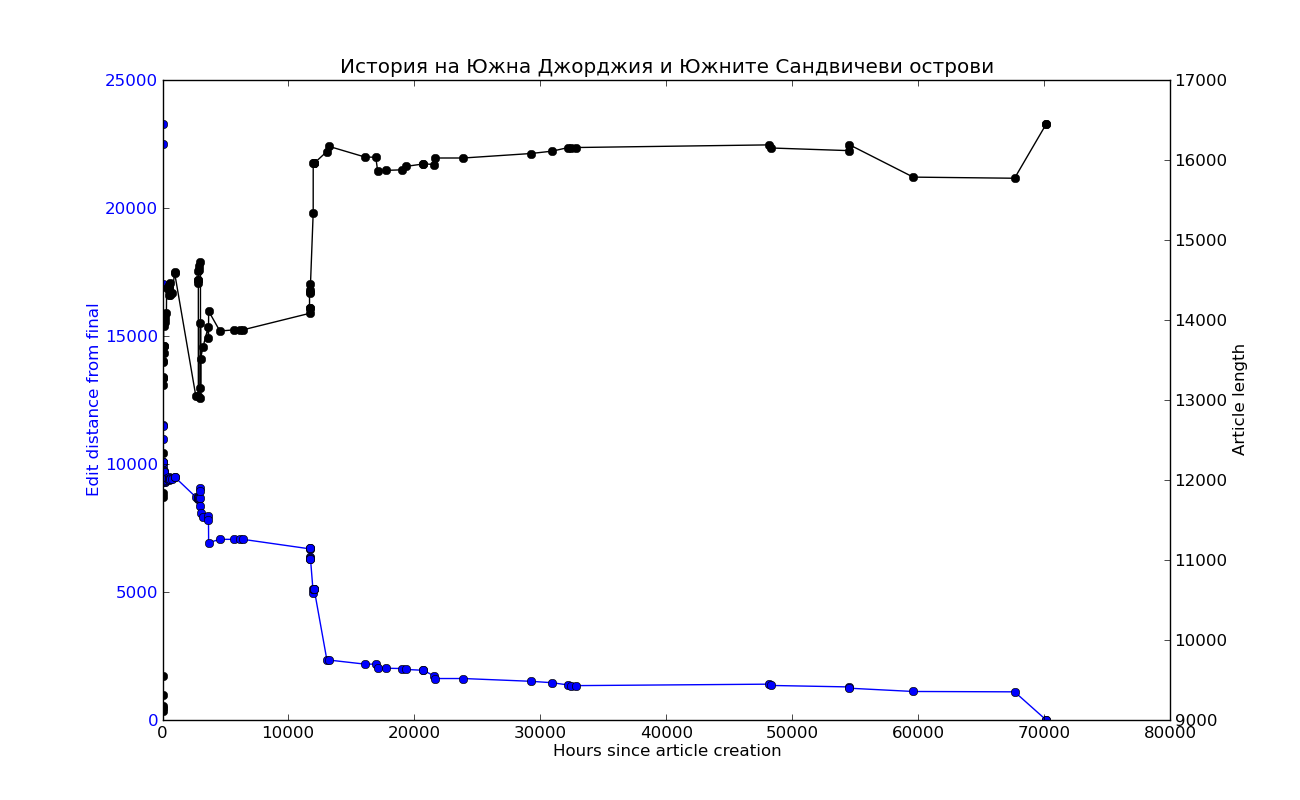
\includegraphics[width=\linewidth]{img/traj-classic/bg90882traj.png}
      \caption{\href{http://bg.wikipedia.org/wiki/index.php?curid=90882}{Bulgarian
          Wikipedia, Page ID 90882 (History of South Georgia and the
          South Sandwich Islands)}}
    \end{subfigure}
    \begin{subfigure}[b!]{0.6\linewidth}
      \centering
      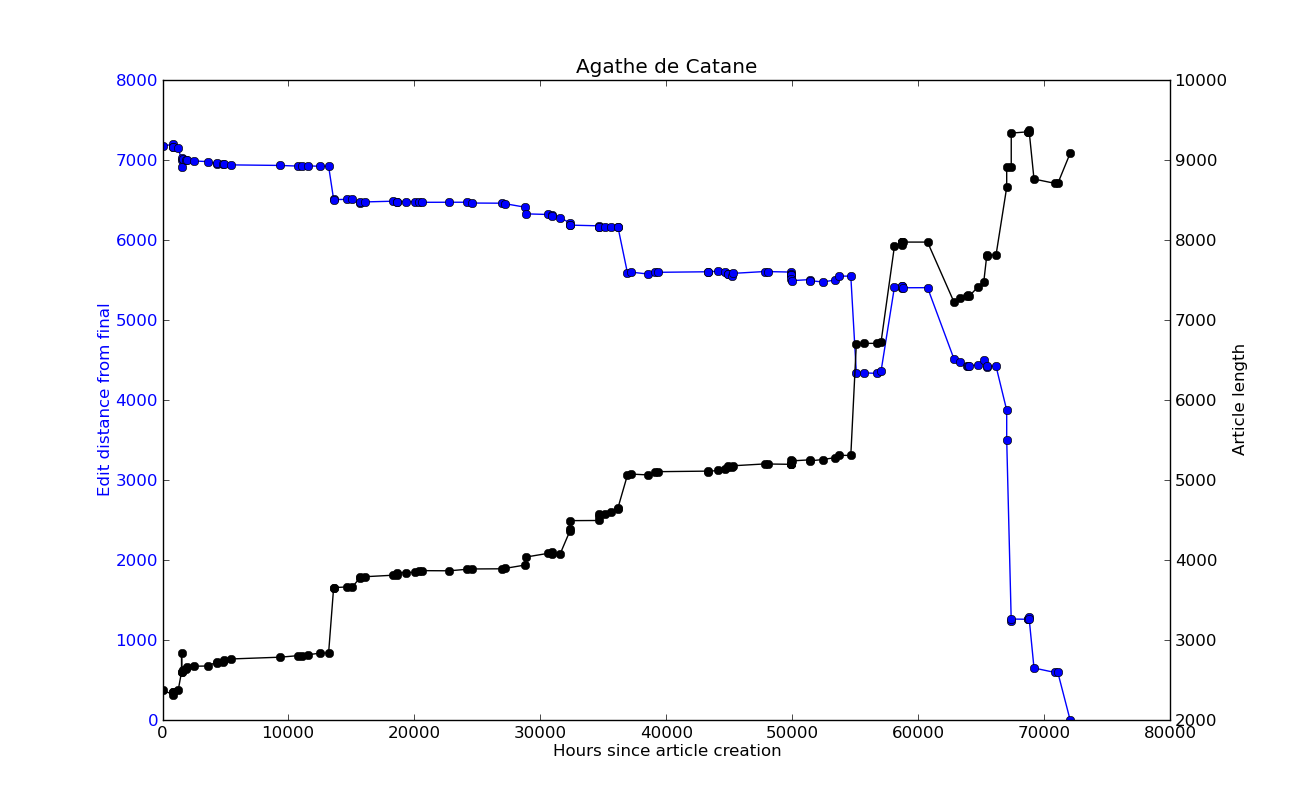
\includegraphics[width=\linewidth]{img/traj-classic/fr572796traj.png}
      \caption{\href{http://fr.wikipedia.org/wiki/index.php?curid=572796}{French
          Wikipedia, Page ID 572796 (Agatha of Catania)}}
    \end{subfigure}
  }\\
  \makebox[\linewidth][c]{
    \begin{subfigure}[b!]{0.6\linewidth}
      \centering
      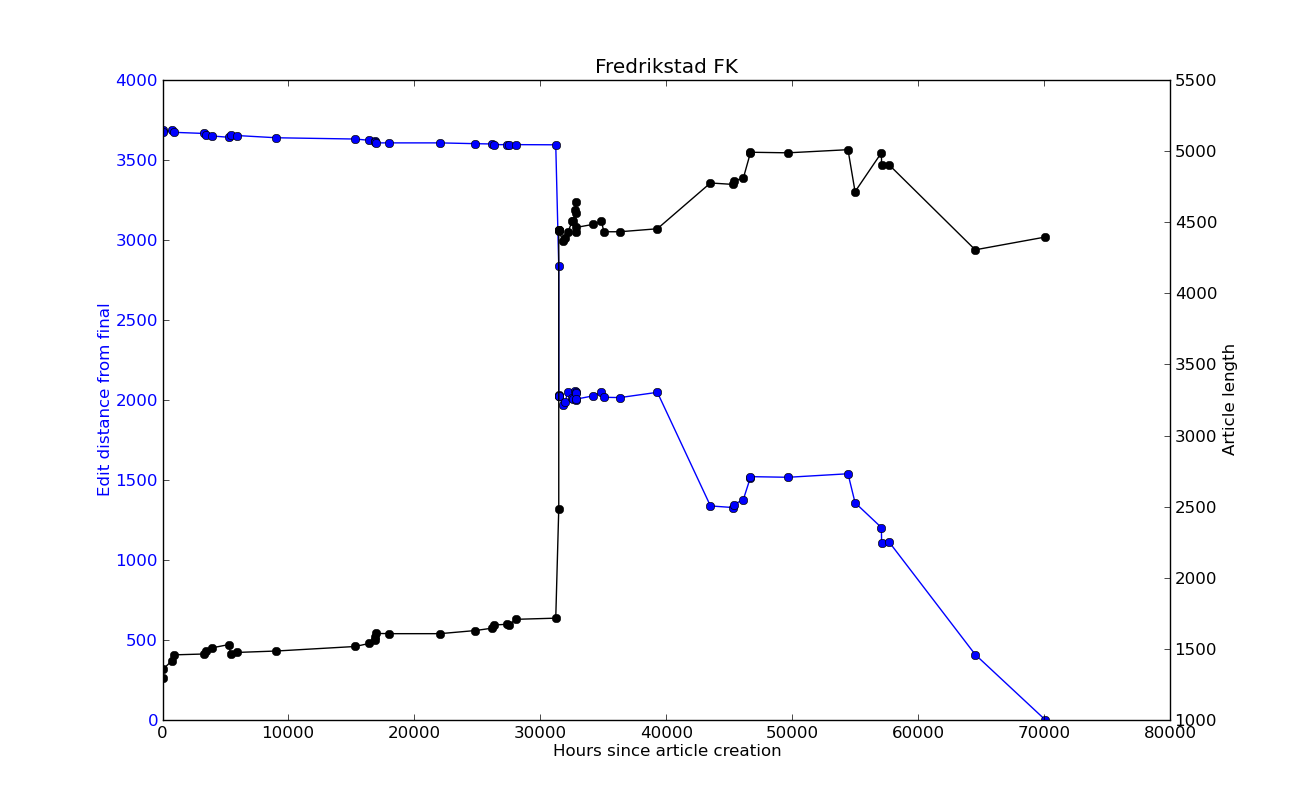
\includegraphics[width=\linewidth]{img/traj-classic/pl291709traj.png}
      \caption{\href{http://pl.wikipedia.org/wiki/index.php?curid=291709}{Polish
          Wikipedia, Page ID 291709 (Fredrikstad FK, a Norwegian
          football club)}}
      \label{fig:fredrikstad}
    \end{subfigure}
    \begin{subfigure}[b!]{0.6\linewidth}
      \centering
      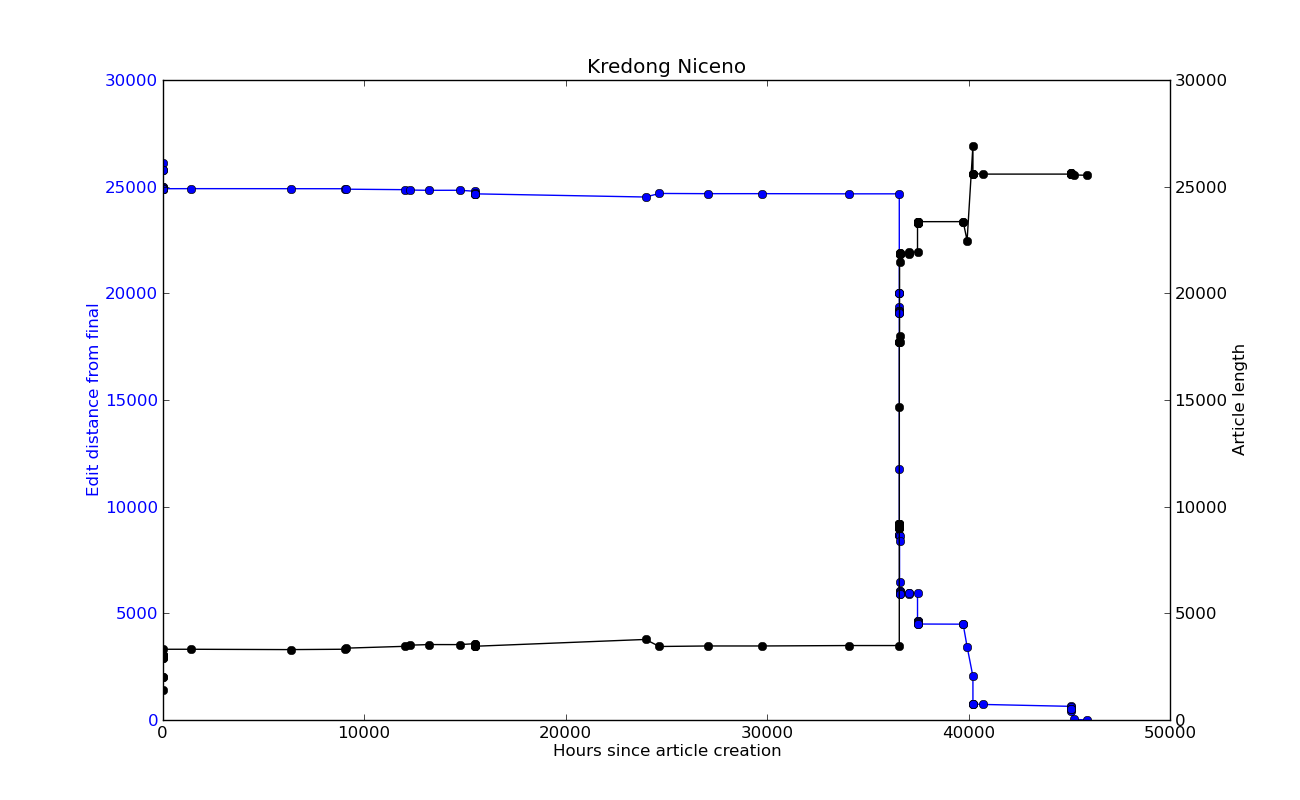
\includegraphics[width=\linewidth]{img/traj-classic/tl62286traj.png}
      \caption{\href{http://tl.wikipedia.org/wiki/index.php?curid=62286}{Tagalog
          Wikipedia, Page ID 62286 (The Nicene Creed)}}
      \label{fig:nicene-creed}
    \end{subfigure}
  }\\
  \makebox[\linewidth][c]{
    \begin{subfigure}[b!]{0.6\linewidth}
      \centering
      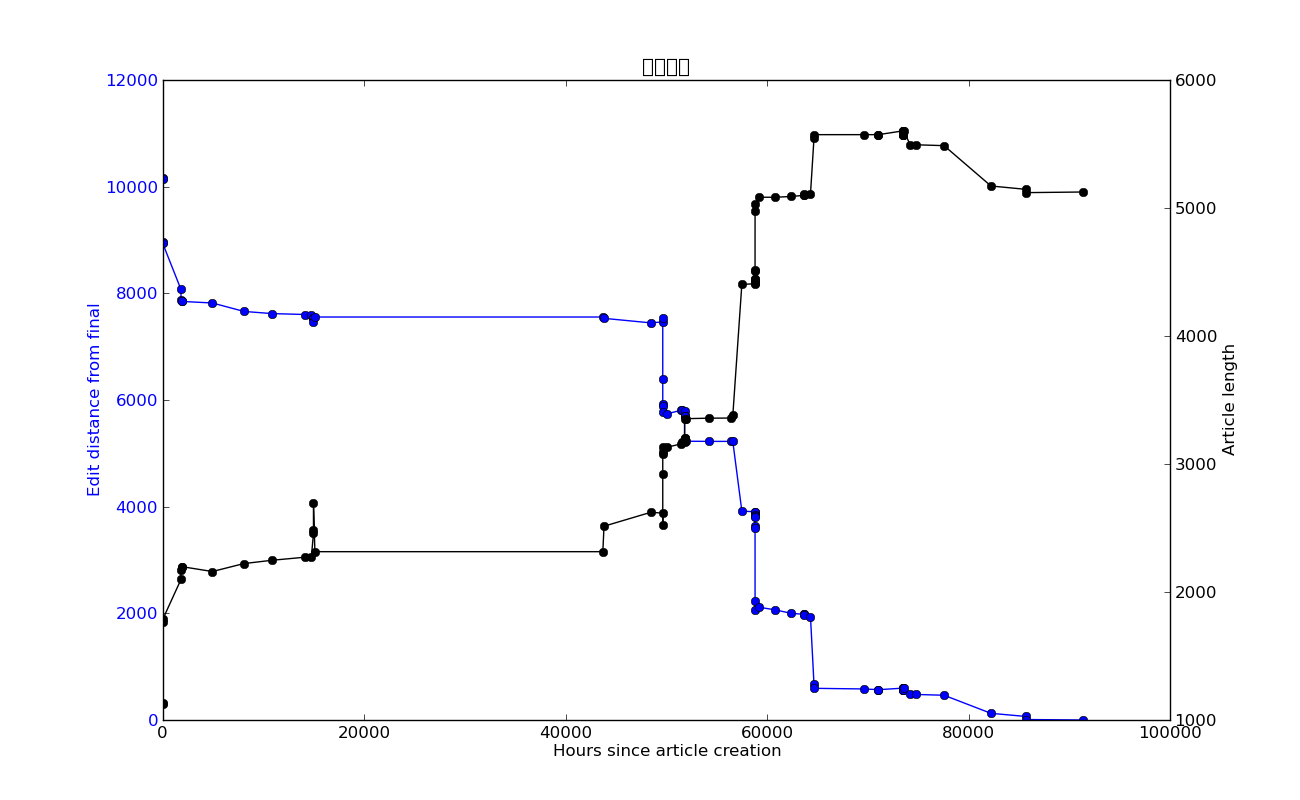
\includegraphics[width=\linewidth]{img/traj-classic/ja1611162traj.png}
      \caption{\href{http://ja.wikipedia.org/wiki/index.php?curid=1611162}{Japanese
      Wikipedia, Page ID 1611162 (The Tax Treaty)}}
      \label{fig:japanese-tax}
    \end{subfigure}
    \begin{subfigure}[b!]{0.6\linewidth}
      \centering
      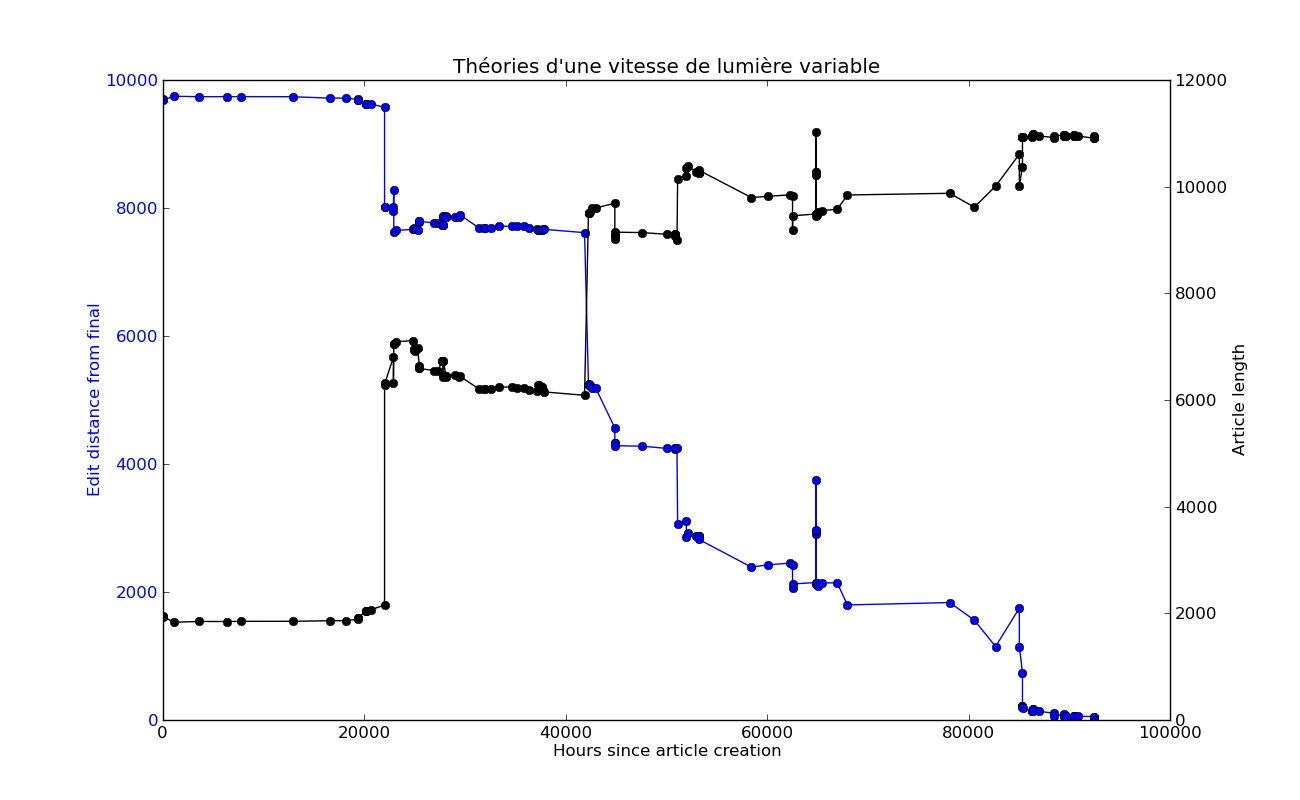
\includegraphics[width=\linewidth]{img/traj-classic/fr43937traj.png}
      \caption{\href{http://fr.wikipedia.org/wiki/index.php?curid=43937}{French
      Wikipedia, Page ID 43937 (Theories of a variable light speed)}}
      \label{fig:variable-light}
    \end{subfigure}
  }
  \caption{Simple trajectory graphs.}
  \label{fig:traj-classic}
\end{figure}

In the last of these simple trajectory graphs we find the first of our
notable features. Figure~\ref{fig:variable-light} shows a clear sign
of an undo operation at around 65,000 into the age of the article. We
see the black line take a steep ascent and immediate descent, showing
a quick enlargement and reduction of the article size. Since the same
spike can be seen in the blue line, we know that inserting this text
made the the article more different from the final version, and the
removed text brought us back. We can infer that the same text that was
added was the same as that which was removed. We find one of these
redo-undo edits
\href{http://fr.wikipedia.org/w/index.php?title=Th\%C3\%A9ories\_d\%27une\_vitesse\_de\_lumi\%C3\%A8re\_variable&diff=96659084&oldid=96654283}{in
  the wikipedia diff between revids 96659084 and 96654283}.

In contrast, the Phillipino article on the Nicene Creed
(Figure~\ref{fig:nicene-creed}) has a similar-shaped spike in it's
size. The event can be seen to occur just after 40000 hours. In this
case however, the trajectory line does not spike in turn. In this case
we can assume that the inserted spike shows an insertion of text that
remains in the article, and the deletion of text that is not
re-inserted before the article's current version.

These spikes are fairly obvious characteristics to identify on plots
such as these. However, we may also identify longer periods of
meandering away from and back towards the current version. Notice the
arced paths in figure~\ref{fig:fredrikstad}, spanning around 45000 to
55000 hours. Although the time frame is much larger than in the other
articles (10,000 hours $\approx$ 1 year 2 months), and multiple edits
occur in the meantime, we may also characterise the overall event as
an `undo' operation. It is more nuanced than others we have identified
so far (after the event the article is equally similar to the current
version, but smaller in size), but the effect is the same. The burden
is upon our model as to how to sufficiently characterise these
long-term removals of useless inserted material.

We also may begin to notice that that edits may tend to cluster in
time, and that the articles may owe much of their content one-time
bursts of activity. The Japanese article on tax
(figure~\ref{fig:japanese-tax}), after an `undo'-shaped cluster of
edits at around 15000 hours, was not edited again for almost 3
years. The Tagalog and Polish articles (respectively the smallest and
largest articles discussed so far) gained most their content over just
a few days. 

Stranger history can be found in the plots in
figure~\ref{fig:traj-bot}. These show another common shape: a slow
climb in both distance-from-final and size, before a sharp drop. The
shape seems to describe an article which engorged with content, before
having the majority of it deleted. On further inspection we found that
the articles generally share two characteristics -- they come from
small Wikipedias, and the majority of the edits are made by bots. We
can see from the user-names on the right-hand side that they are bots
-- there is a special bot `flag' to be raised in the user profile of
bots, but it is also traditional for the bot to be also be given an
identifying name.\cite{wiki-bot-policy}
 
\begin{figure}
  \centering
  \makebox[\linewidth][c]{
    \begin{subfigure}[b!]{1.2\linewidth}
      \centering
      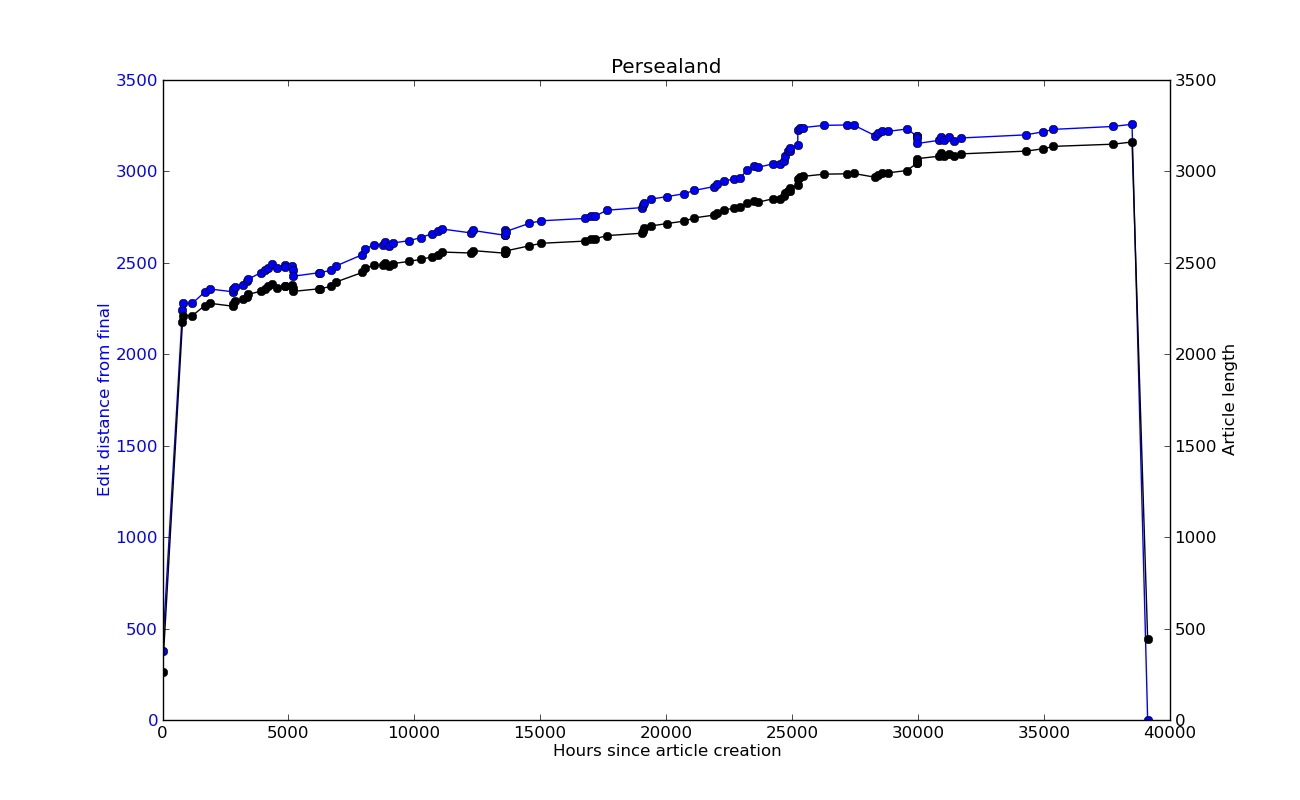
\includegraphics[width=0.45\linewidth]{img/traj-bot/ang7120traj.png}
      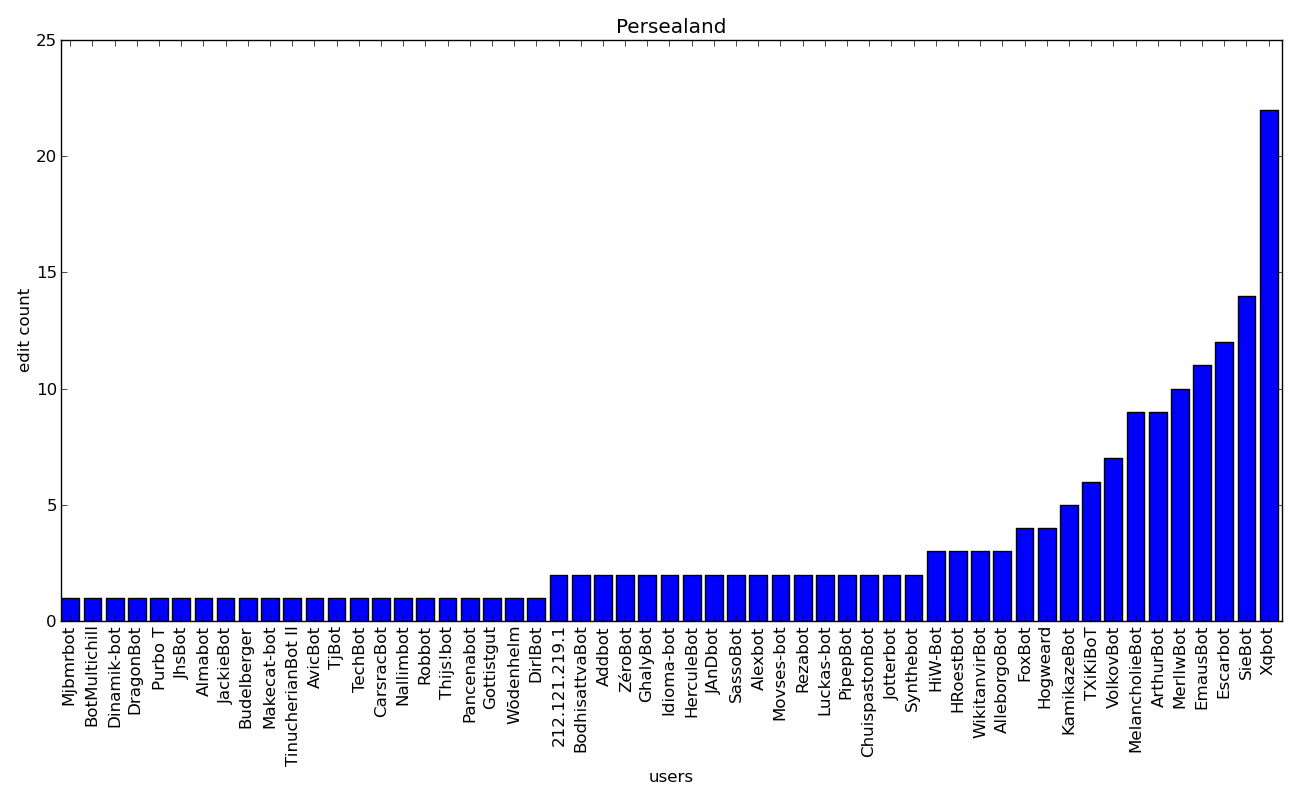
\includegraphics[width=0.45\linewidth]{img/traj-bot/ang7120users.png}
      \caption{\href{http://ang.wikipedia.org/wiki/index.php?curid=7120}{Anglo-Saxon
          Wikipedia, Page ID 7120 (Persia)}}
    \end{subfigure}
  }\\
  \vspace{5mm}
  \makebox[\linewidth][c]{
    \begin{subfigure}[b!]{1.2\linewidth}
      \centering
      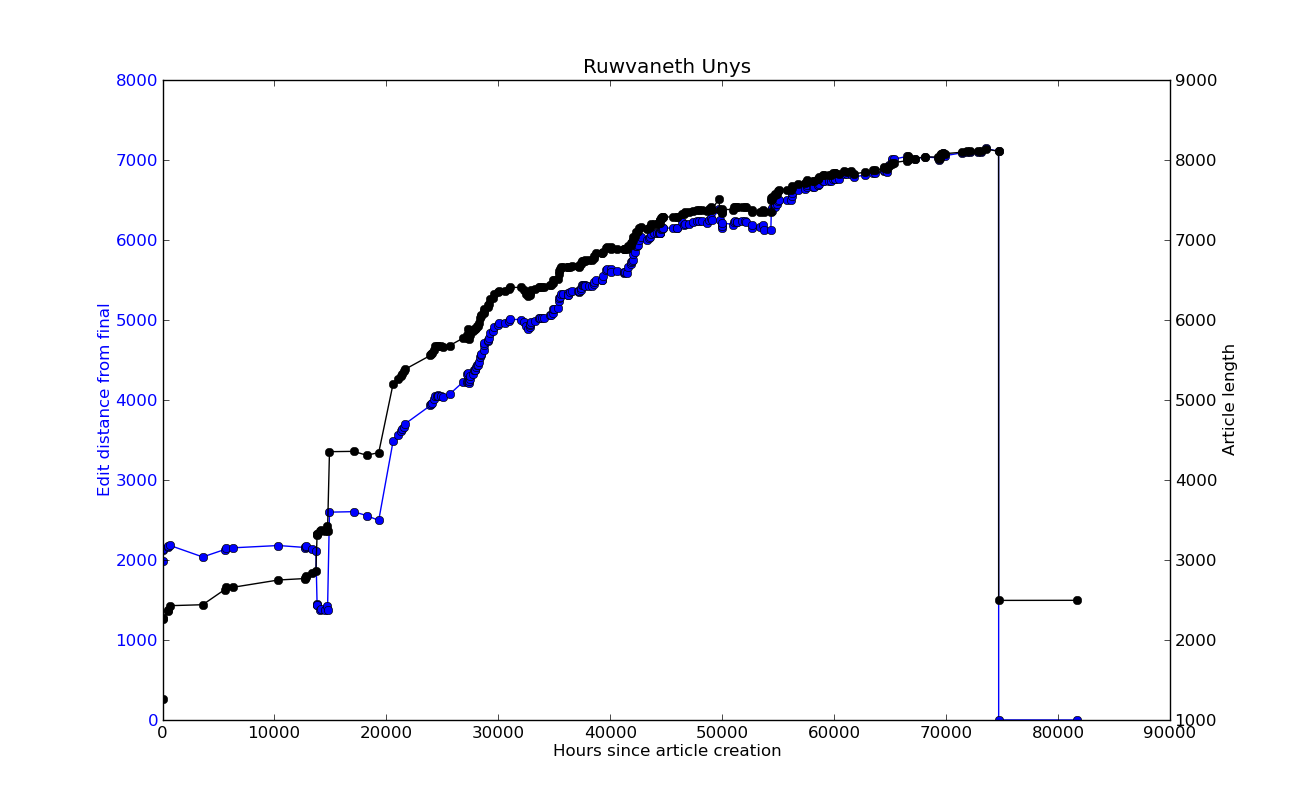
\includegraphics[width=0.45\linewidth]{img/traj-bot/kw736traj.png}
      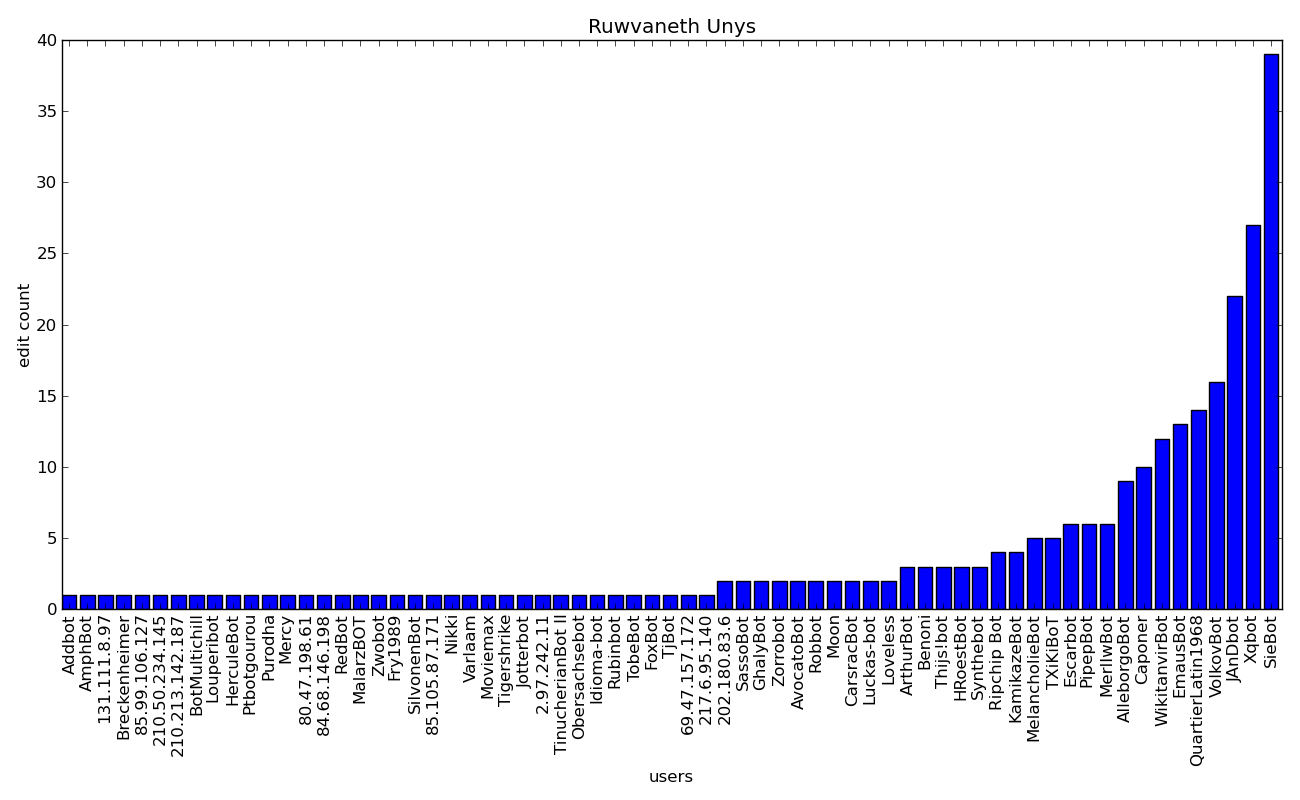
\includegraphics[width=0.45\linewidth]{img/traj-bot/kw736users.png}
      \caption{\href{http://kw.wikipedia.org/wiki/index.php?curid=736}{Cornish
          Wikipedia, Page ID 726 (United Kingdom)}}
    \end{subfigure}
  }\\
  \vspace{5mm}
  \makebox[\linewidth][c]{
    \begin{subfigure}[b!]{1.2\linewidth}
      \centering
      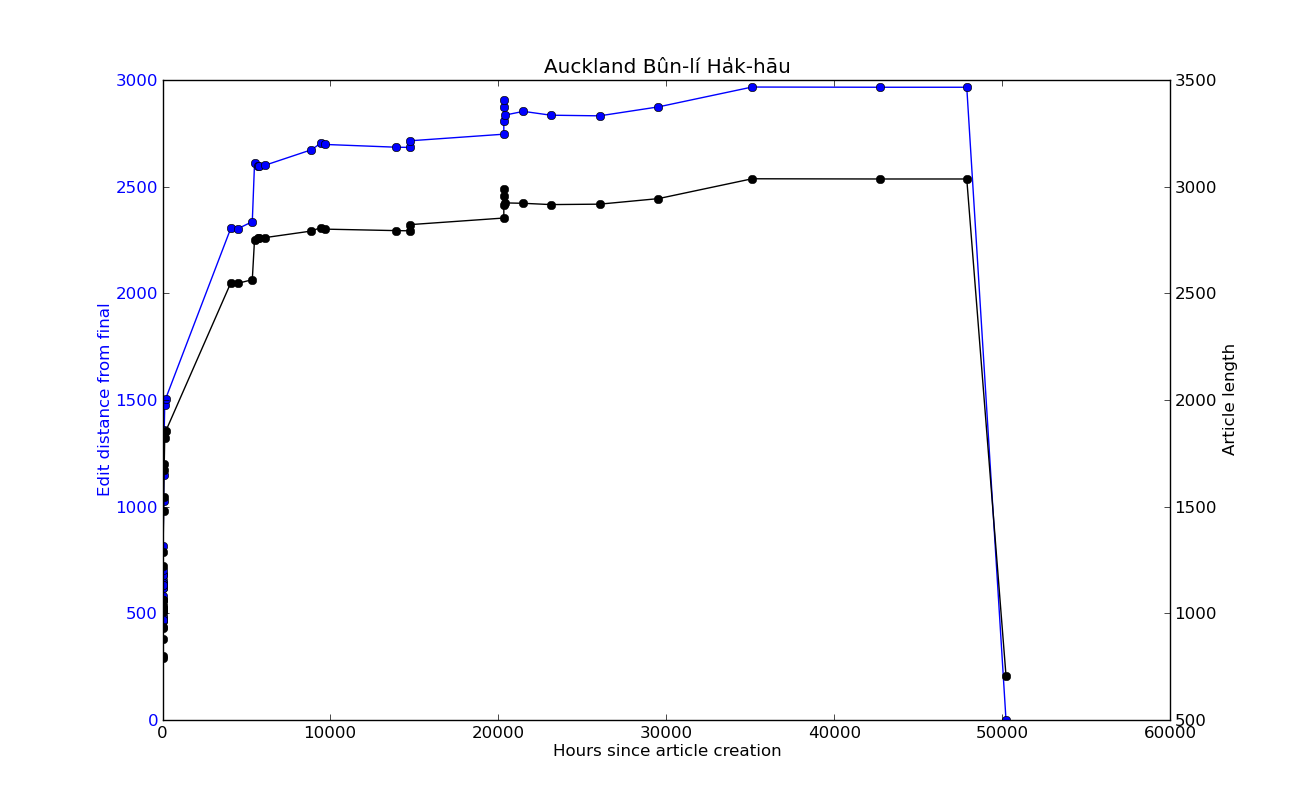
\includegraphics[width=0.45\linewidth]{img/traj-bot/zh-min-nan10733traj.png}
      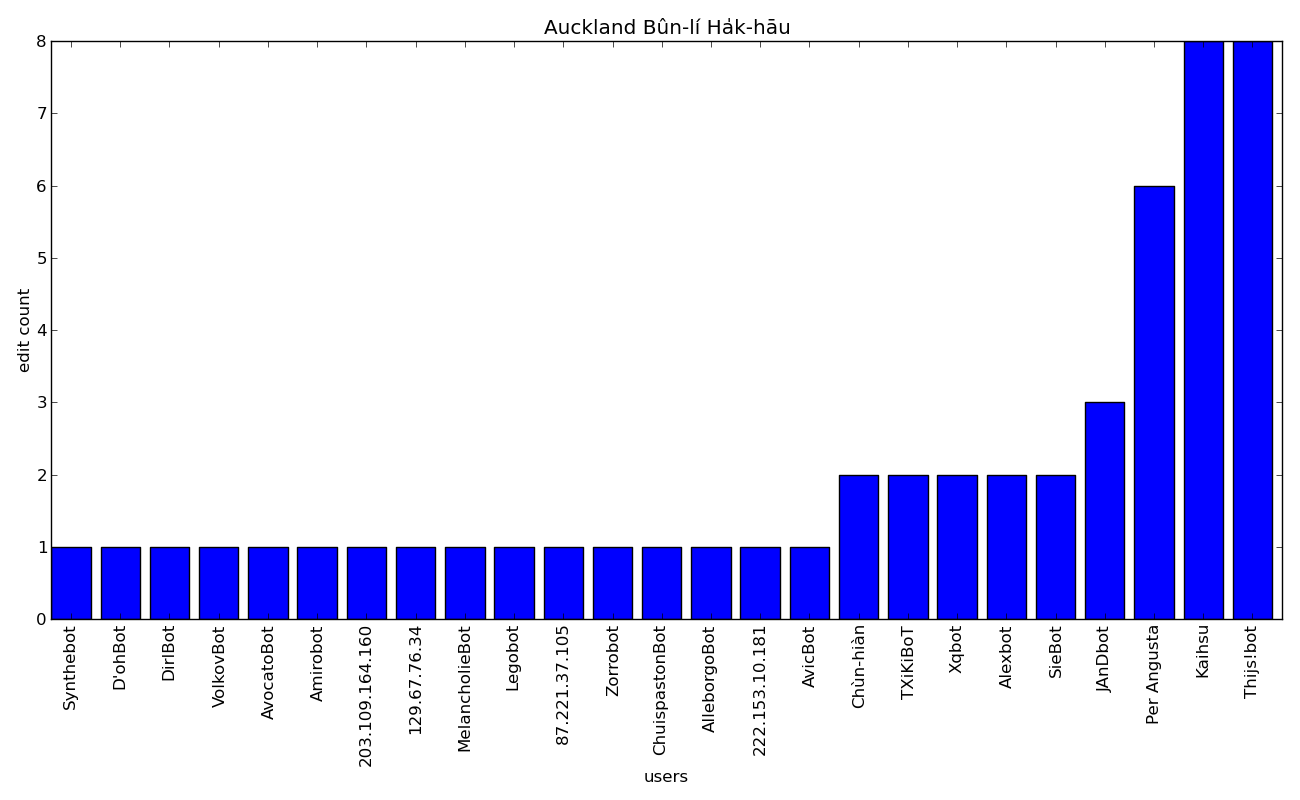
\includegraphics[width=0.45\linewidth]{img/traj-bot/zh-min-nan10733users.png}
      \caption{\href{http://zh-min-nan.wikipedia.org/wiki/index.php?curid=10733}{Min
          Nan Wikipedia, Page ID 10733 (Auckland Grammar School)}}
    \end{subfigure}
  }\\
  \caption{Trajectory graphs showing bot editing characteristics.}
  \label{fig:traj-bot}
\end{figure}

The explanation is in the articles' histories. In each one, we find a
single large deletion event, occurring any time after early 2013. With
a little digging, we find the origin of the act to be a Wikimedia
project that aims to `migrating inter-language wiki links from
individual articles into a central database to ease
maintenance',\cite{wiki-interwikilinks} see
figure~\ref{fig:traj-bot-explanation} for the native wiki diff of just
one of these events. Each wikipedia article is rendered to the right
of a language bar that links that article to its counterpart in
various languages. Once coded into each article manually, these links
are now stored in and served dynamically from a central
source.\cite{wiki-blog-onwikidata} The move gives us strange results
for this project -- for small articles, the loss of these hard-coded
links constitutes a gutting of its majority content. By our
measurements, in these circumstances, this act of housekeeping is a
momentous event in the history of small articles.

\begin{figure}
  \centering \makebox[\linewidth][c]{
    \begin{subfigure}[b!]{1.2\linewidth}
      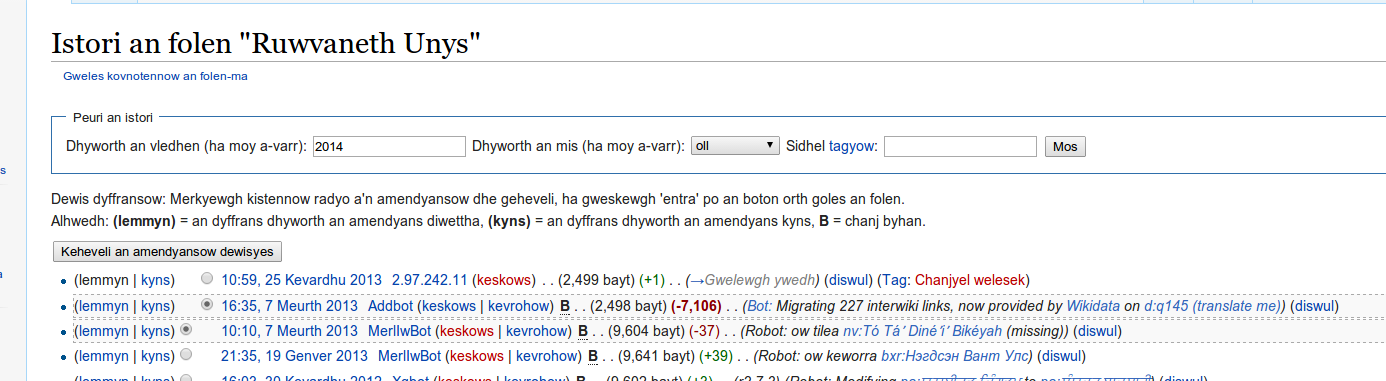
\includegraphics[width=1\linewidth]{img/traj-bot/botmigration.png}
      \caption{Migration event in article history (16:35, 7 March
        2013)}
    \end{subfigure}
  }\\ 
  \vspace{8mm}
  \makebox[\linewidth][c]{
    \begin{subfigure}[b!]{1.2\linewidth}
      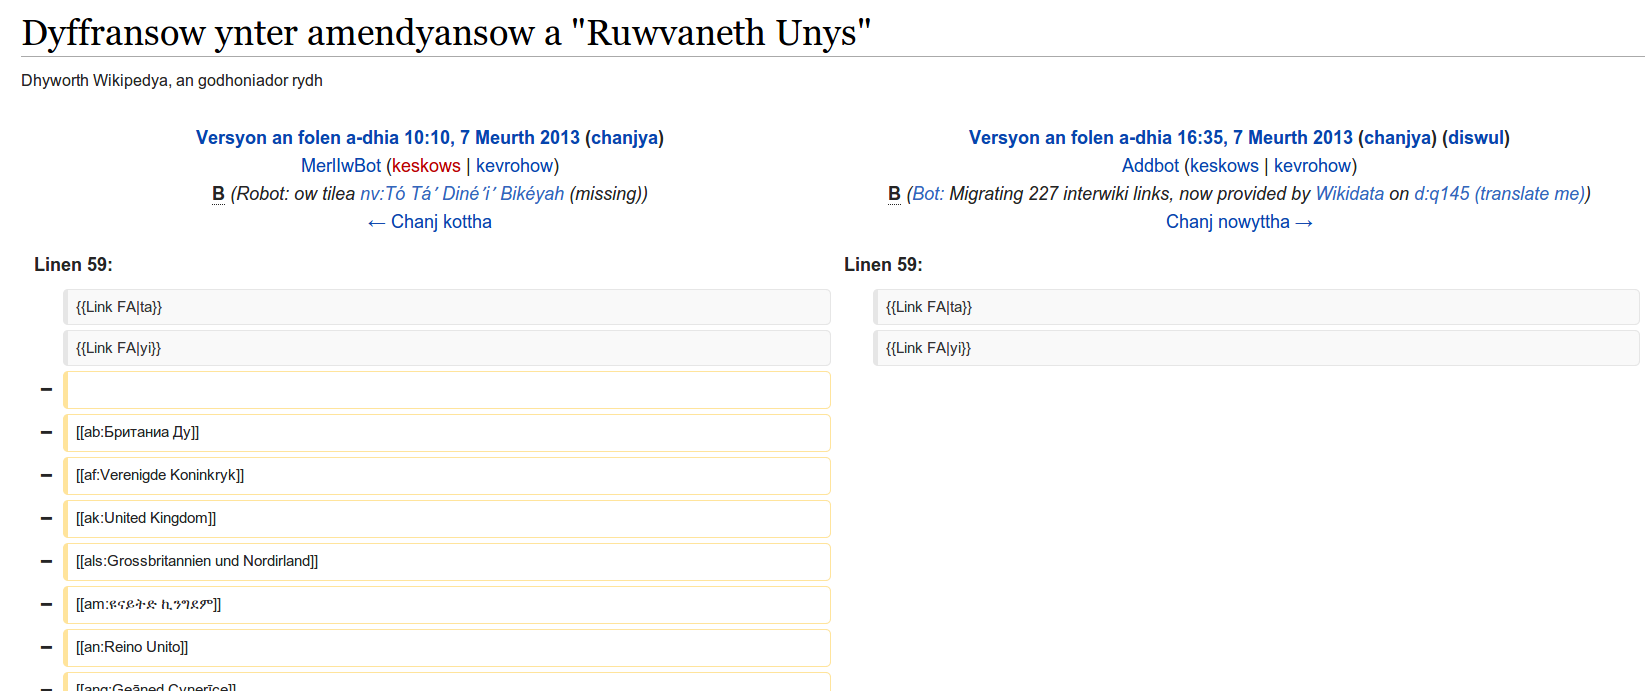
\includegraphics[width=1\linewidth]{img/traj-bot/botdiff.png}
      \caption{The Wikipedia diff for the migration event}
    \end{subfigure}
  }
\caption{Screenshots showing automated migration of inter-language
  links.}
\label{fig:traj-bot-explanation}
\end{figure}

How do we characterise this? In this case the `article', as such, is
unchanged. Indeed the rendered page is identical before and after the
link cull. We may think to ignore bot edits to a page, but how do we
distinguish between the addition and deletion of these language links
from meaningful changes to content? We may distinguish from, say,
useful spell-checking bots by means of a simple text regex (inter-wiki
links always have the same form), but we may not as easily distinguish
language-bar links from in-line ones -- those that may link to related
articles, rather than mirror articles, widening knowledge rather than
offering what may merely be a translation of the original
article. We discuss this later.

\subsection*{Combining trajectory plots}
Derek Smart's wikipedia page has been named as the battleground of one
of the `lamest WikiWars' -- it is the place where a very long argument
about whether or not to include criticisms of his work on his page.
We use it here as a case study for how derive more information about
the context of a page with our tools.

In figure~\ref{fig:dsmart-case} we see the combination of trajectory
plots on three different pages -- the green and black lines represent
the same article trajectory / article size we've looked at previously,
but accompanying those we have plots of the talkpage for that article,
and the page detailing the arbitration request raised for that page. 

We see clearly page's activity density is relative to the density on
the respective talk page. We also see that a large part of the
article's history follows the same large-unnecessary-growth pattern we
recognised in the small, bot-dominated pages analysed previously. By
the end of the densest period, the page is much smaller, and is
quite dissimilar from the article state at the height of activity.

But perhaps the most interesting part of this graph is the plot of the
request for arbitration page -- the blue line. We see it created at
the height of the page's size and from-final dissimilarity, and during
a particularly turbulent patch of the talk page history. We also see
that as the arbitration page reaches it's final versions (the decision
on the dispute), the commotion begins to cease, the page
shortens, is edited less frequently, and approaches it's final version
quite quickly.

\begin{figure}[p]
  \centering
  \makebox[\linewidth][c]{
    \begin{subfigure}[b!]{1.2\linewidth}
      \centering
      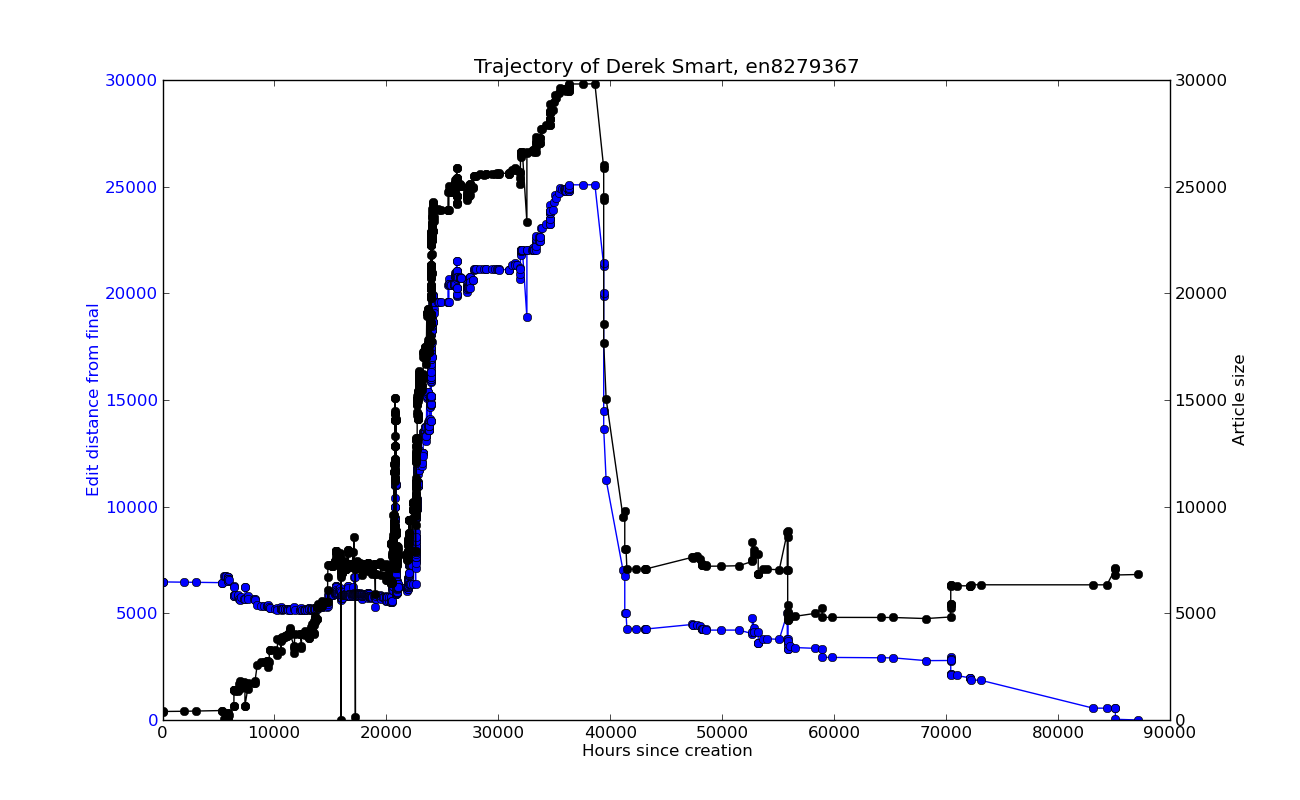
\includegraphics[width=0.3\linewidth]{img/dsmart/dereksmarttraj.png}
      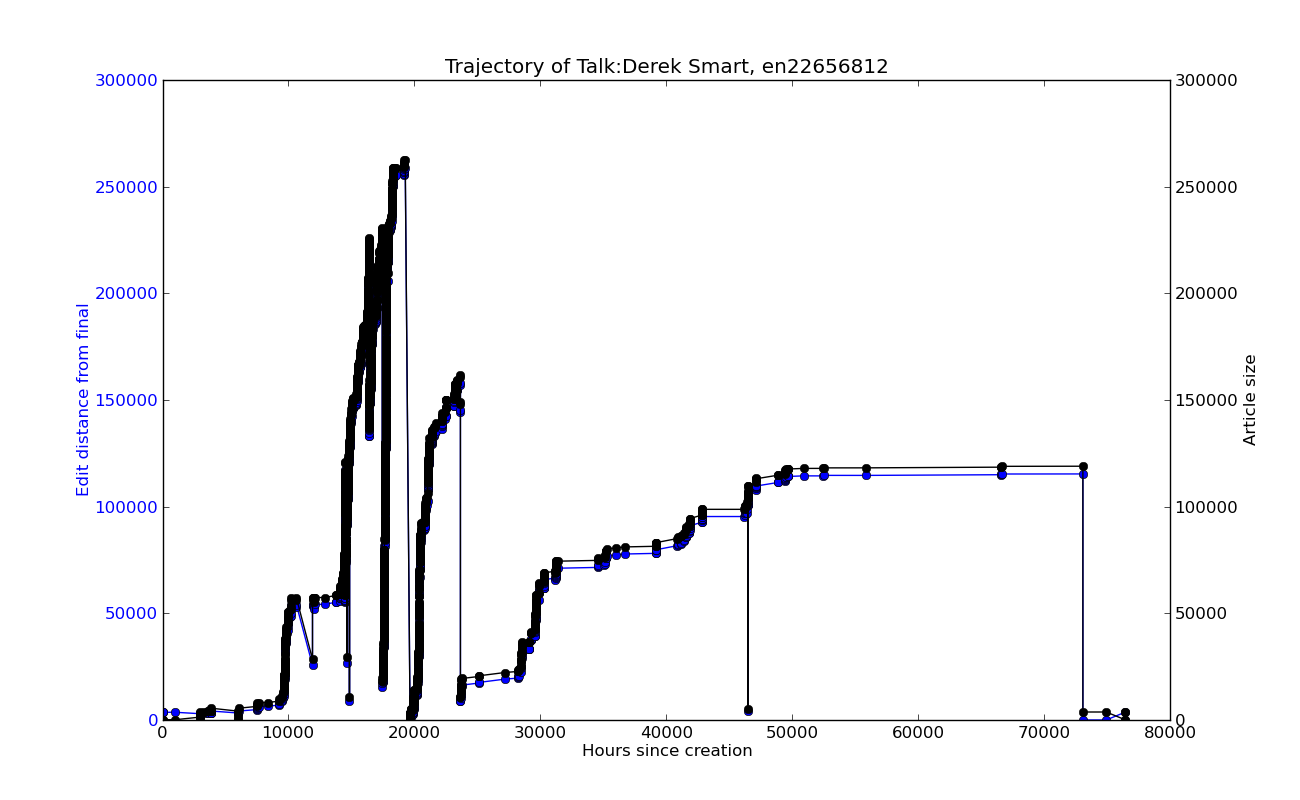
\includegraphics[width=0.3\linewidth]{img/dsmart/dereksmarttalk.png}
      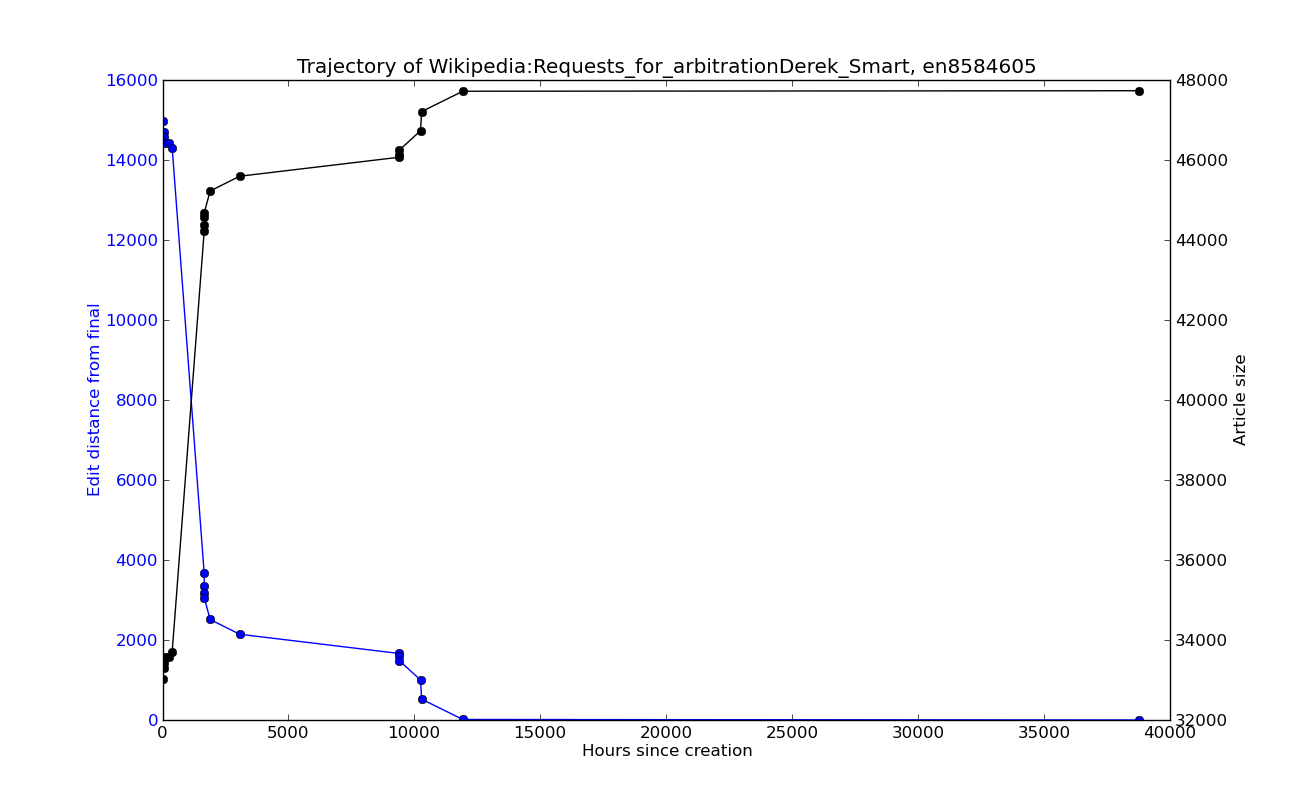
\includegraphics[width=0.3\linewidth]{img/dsmart/dereksmartarbritration.png}
    \end{subfigure}
  }\\
  \makebox[\linewidth][c]{
    \begin{subfigure}[b!]{1.2\linewidth}
      \centering
      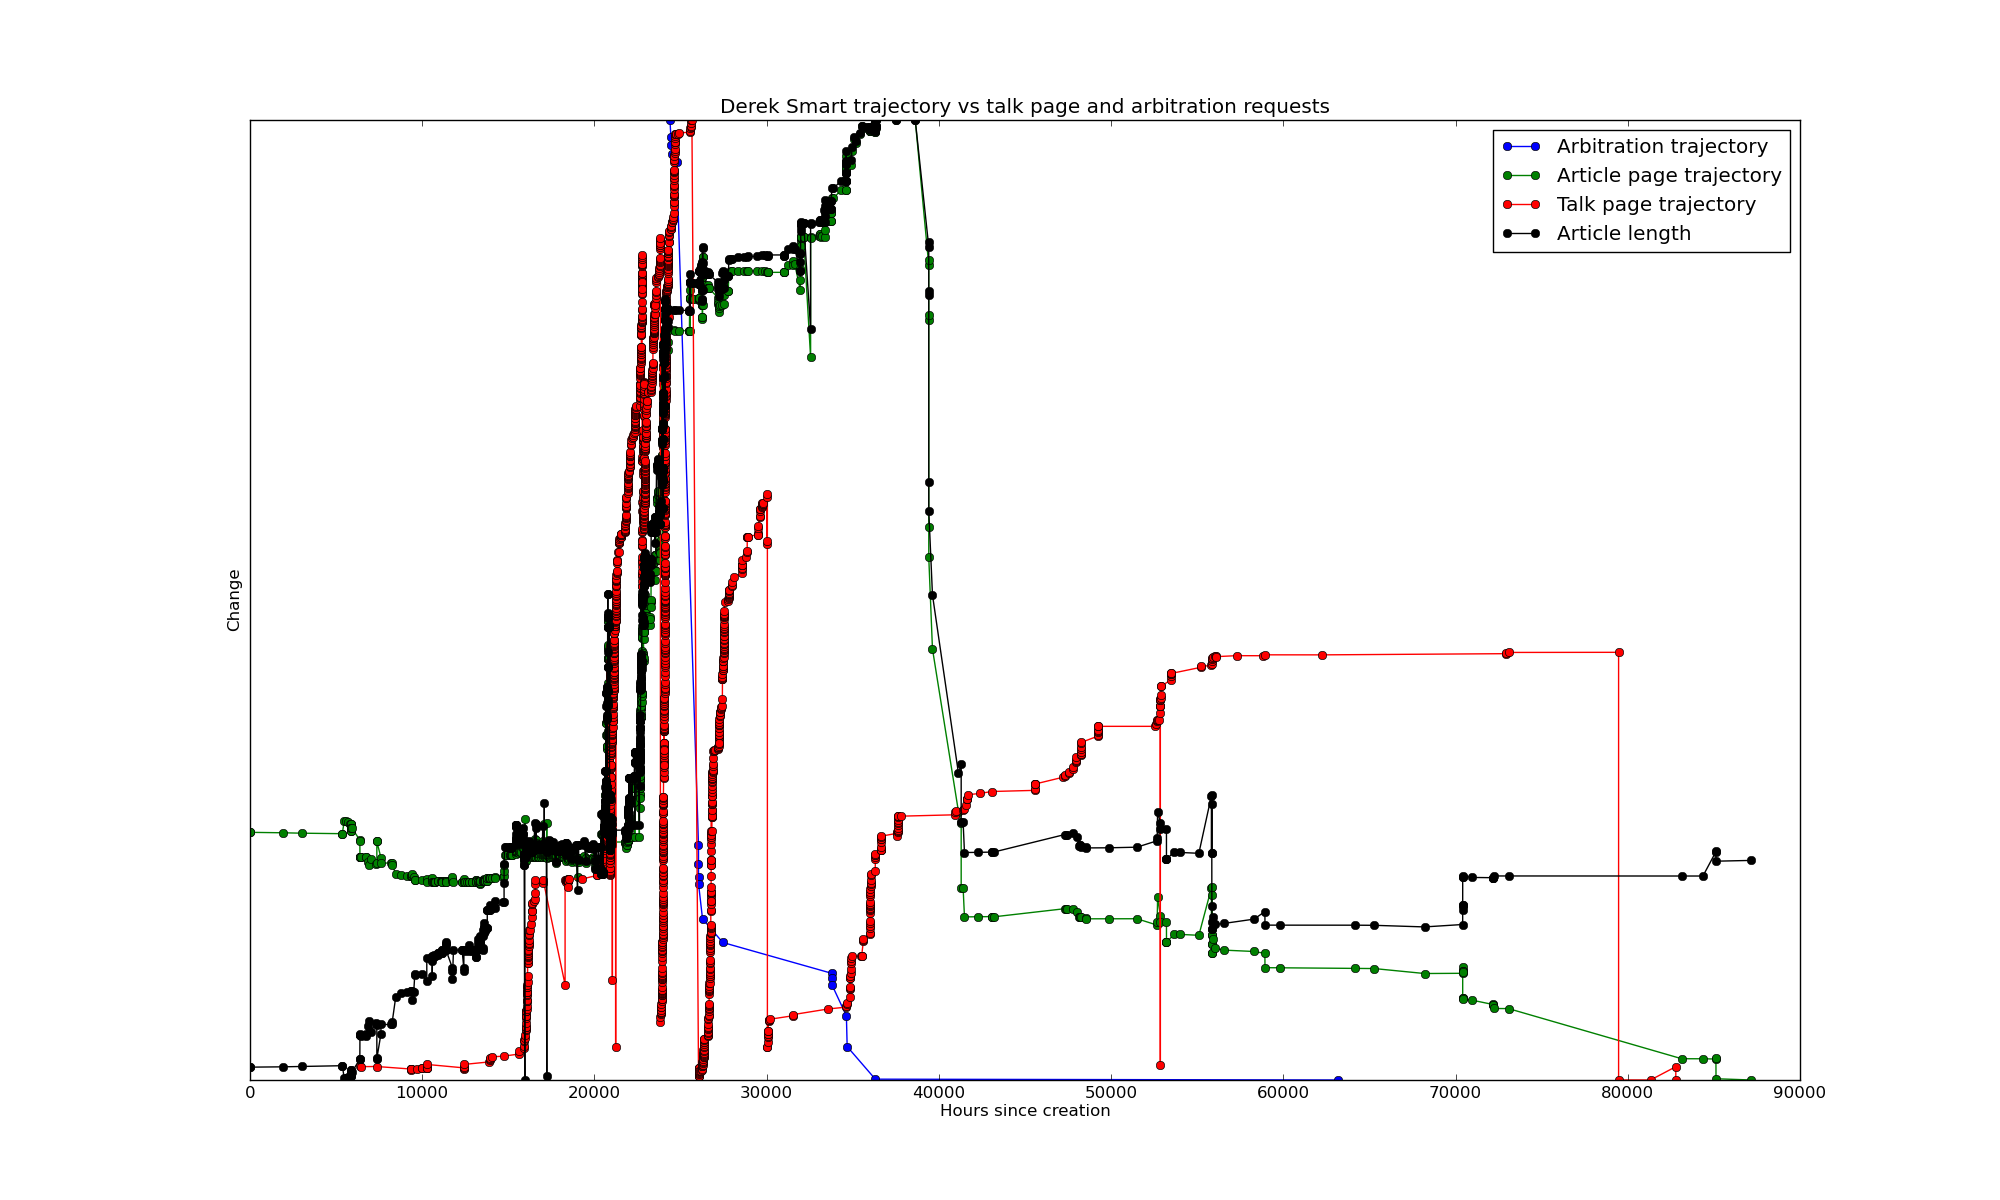
\includegraphics[width=1\linewidth]{img/dsmart/dereksmartcombo.png}
      \caption{\href{http://kw.wikipedia.org/wiki/index.php?curid=736}{Cornish
          Wikipedia, Page ID 726 (United Kingdom), normalised y-axis
          values}}
    \end{subfigure}
  }\\
  \caption{Obtaining greater context of an article's history by
    combining page trajectories}
  \label{fig:dsmart-case}
\end{figure}

In this particular case, a small handful of members were arguing about
whether or not to include criticisms on Derek Smart and his work in
his article. At the height of the argument, they involved parties
called for an arbitration committee to help resolve the issue. The
article was ``urgently referred to the Wikipedia editing community at
large for cleanup, evaluation of sources, and adherence to
[Neutral Point of View]'', as well as restrictions on who could edit
the article, and how.

So perhaps it would be important for us to reward editors who
participate in these discussions accordingly. With simple arithmetic
operations we can see when an argument has turned out to be eventually
irrelevant to a document's final version -- we see that this one
involved the addition of a lot of eventually removed text -- and
perhaps penalise the key editors involved by cross-referencing their
edits between the pages. We can also see when the opposite occurs. The
downward slope of the graph in figure~\ref{fig:dsmart-case}
perhaps shows a reconciliation, and efforts to change the article
according to the conclusions of the article. We may see if the arguing
editors are involved in this `tidying', and regard them accordingly.

In any case we see that the immediate context of a page can have great
effects on the path nature of the collaboration, as well as the final
product.

We find a similar case in the biographical article for English
biologist Rupert Sheldrake. Rupert Sheldrake, whose `astonishingly
visionary' early work in plant science had him described as `one of
the brightest Darwinians of his
generation',\cite{odyssey-auxin}\cite{guardian-shel}, came under heavy
criticism for his later work in psychical research, and `mysterious
telepathy-type interconnections between organisms and collective
memories within species'.\cite{sheldrake-biog}

\begin{figure}
  \centering
  \centering
  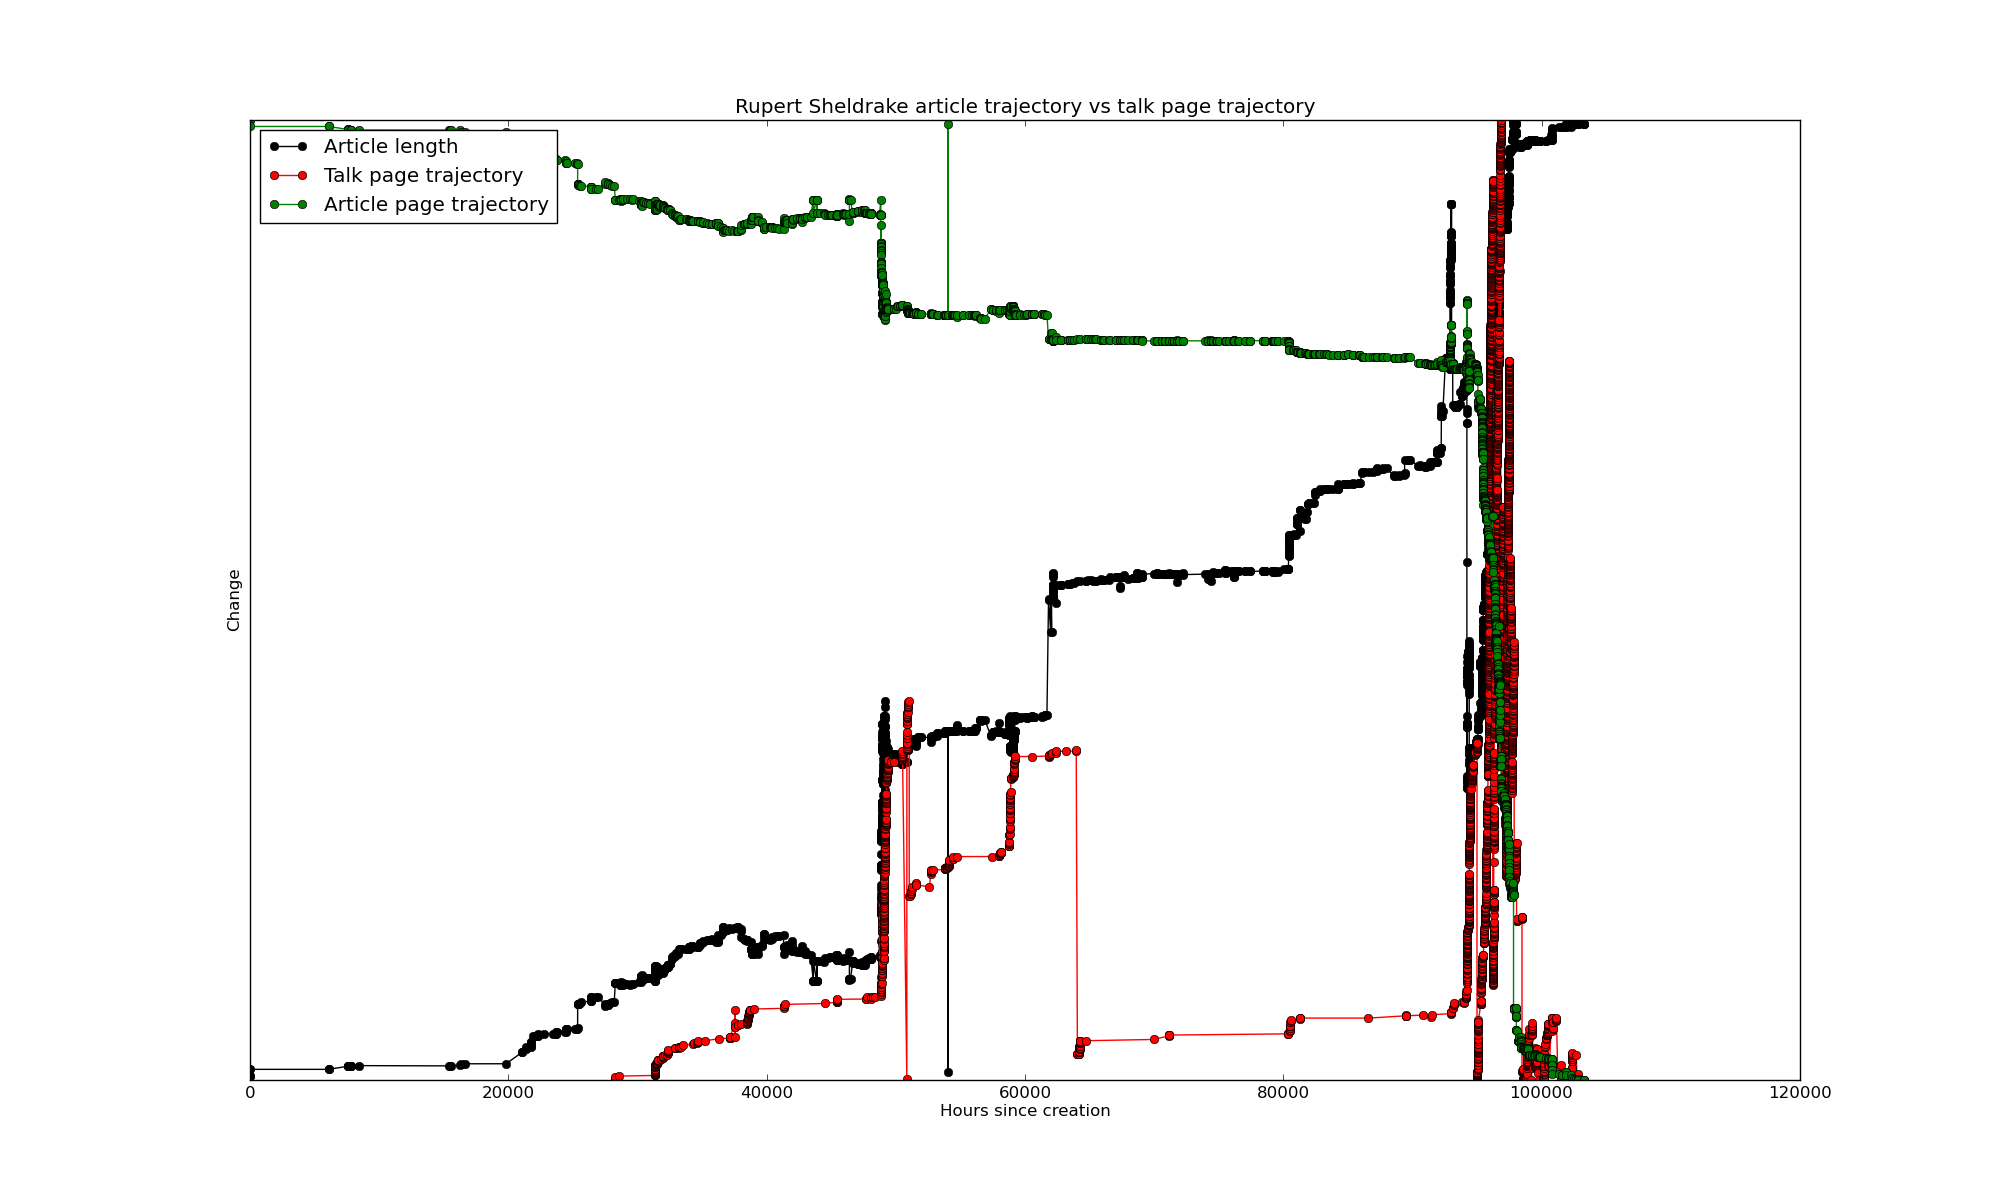
\includegraphics[width=\linewidth]{img/rsheldrake/RupertSheldrakecombo.png}
  \caption{English Wikipedia, page ID 142395 (Rupert Sheldrake),
    article vs talk page trajectory graph}
  \label{fig:sheldrake-plot}
\end{figure}

Figure~\ref{fig:sheldrake-plot} shows a graph similar to the Derek
Smart plot, though a request for arbitration has not yet been made. In
fact, though it's history is already quite dense, it has only been in
the last year-or-so that the activity has really started, and we can
expect this graph to look quite different if recalculated in a few
months.

This spike in activity is a result of direct publicity. Rupert
Sheldrake has been controversial for years (in 1981, Nature wrote of
one of his works that it was `a book for burning'), so it is not
surprising to see arguments surface here. 

But on Wikipedia, we may see that the activity peak is associated with
something slightly different --- provoking regular editors by
questioning the their possibly overpowering predilections towards
certain opinions. In November 2013, Rupert Sheldrake accused
`guerilla' editors of ``distorting hundreds of pages on
Wikipedia''\cite{sheldrake-bbc-interview}, and the argument started
from there. One of the key players in the ensuing argument on
Wikipedia began his own website about the possible problem, in
reaction to his percieved abuse. It is called `Wikipedia, we have a
problem'.\cite{wiki-problem}

We consider, then, that the context of these edits may not simply be
edit count, density of talk, but a page may also be greatly affected
the unpredictable whims of editors, that the trajectory of a page may
be shaped by a conflict of opinions, rather than facts.
